\documentclass[
	% -- opções da classe memoir --
	12pt,				% tamanho da fonte
	openright,			% capítulos começam em pág ímpar (insere página vazia caso preciso)
	oneside,			% para impressão em verso e anverso. Oposto a oneside
	a4paper,			% tamanho do papel. 
	% -- opções da classe abntex2 --
	%chapter=TITLE,		% títulos de capítulos convertidos em letras maiúsculas
	%section=TITLE,		% títulos de seções convertidos em letras maiúsculas
	%subsection=TITLE,	% títulos de subseções convertidos em letras maiúsculas
	%subsubsection=TITLE,% títulos de subsubseções convertidos em letras maiúsculas
	% -- opções do pacote babel --
	english,			% idioma adicional para hifenização
	french,				% idioma adicional para 
	hifenização
	spanish,			% idioma adicional para hifenização
	brazil				% o último idioma é o principal do documento
	]{abntex2}


% --- 
% CONFIGURAÇÕES DE PACOTES
% --- 
% ---
% Pacotes básicos 
% ---
\usepackage{lmodern}			% Usa a fonte Latin Modern			
\usepackage[T1]{fontenc}		% Selecao de codigos de fonte.
\usepackage[utf8]{inputenc}		% Codificacao do documento (conversão automática dos acentos)
\usepackage{lastpage}			% Usado pela Ficha catalográfica
\usepackage{indentfirst}		% Indenta o primeiro parágrafo de cada seção.
\usepackage{color}				% Controle das cores
\usepackage{graphicx}			% Inclusão de gráficos
\usepackage{microtype} 			% para melhorias de justificação
\usepackage{ufc-abntex2}
\usepackage{algorithm}			% Para escrever algoritmos
\usepackage{algorithmic}		% Para escrever algoritmos
%\usepackage[font=small,labelfont=bf]{caption}			% Remove as imagens do appencia da lista
\usepackage{subcaption}
%\usepackage{setspace} 			% Definir o espaçamento entrelinhas
%\usepackage{tocloft} 			% Ajustar identação do sumario.
\usepackage{fancyvrb}
%\usepackage{fancyhdr}
\usepackage{caption}
% Modificando o idioma do título de Algoritmos.
\makeatletter
\renewcommand{\listalgorithmname}{Lista de Algoritmos}
\makeatother
% Modificando o caption do algoritmo
\floatname{algorithm}{Algoritmo}
% Modificando o comentário do algoritmo
%\renewcommand{\algorithmiccomment}[1]{\hskip2em$\triangleright$ #1}	
\renewcommand{\algorithmiccomment}[1]{\hfill \(\triangleright\) #1}
% comando configurar a legenda da sub-figura.
\captionsetup[subfigure]{labelfont=bf,textfont=normalfont,singlelinecheck=off,justification=raggedright}
\captionsetup{tablename=Quadro}
\captionsetup[figure]{labelfont=bf,font=small}
% {}---
% Pacotes adicionais, usados apenas no âmbito do Modelo Canônico do abnteX2
% ---
\usepackage{lipsum}				% para geração de dummy text
% ---

% ---
% Pacotes de citações
% ---
\usepackage[brazilian,hyperpageref]{backref}	 % Paginas com as citações na bibl
\usepackage[alf]{abntex2cite}	% Citações padrão ABNT

% ---
% Configurações do pacote backref
% Usado sem a opção hyperpageref de backref
%\renewcommand{\backrefpagesname}{Citado na(s) página(s):~}
% Texto padrão antes do número das páginas
%\renewcommand{\backref}{}
% Define os textos da citação
\renewcommand*{\backrefalt}[4]{
	}%
% ---

% ---
% Configurações de aparência do PDF final

% alterando o aspecto da cor azul
\definecolor{blue}{RGB}{41,5,195}

% informações do PDF
\makeatletter
\hypersetup{
     	%pagebackref=true,
		pdftitle={\@title}, 
		pdfauthor={\@author},
    	pdfsubject={\imprimirpreambulo},
	    pdfcreator={LaTeX with abnTeX2},
		pdfkeywords={abnt}{latex}{abntex}{abntex2}{trabalho acadêmico}, 
		colorlinks=true,       		% false: boxed links; true: colored links
    	linkcolor=black,          	% color of internal links
    	citecolor=black,        		% color of links to bibliography
    	filecolor=magenta,      		% color of file links
		urlcolor=black,
		bookmarksdepth=4
}
\makeatother
% --- 

% --- 
% Espaçamentos entre linhas e parágrafos 
% --- 

% O tamanho do parágrafo é dado por:
\setlength{\parindent}{1.3cm}

% Controle do espaçamento entre um parágrafo e outro:
\setlength{\parskip}{0.2cm}  % tente também \onelineskip


%\usepackage{titlesec}
%\usepackage{titletoc}
	%\begin{Verbatim}[showspaces=false,fontsize=\small]
	%Fonte: Autoria Própria.
	%\end{Verbatim}

\addto\captionsbrazil{
	\renewcommand{\contentsname}
	{\textbf{\fontsize{12}{12}\selectfont {SUMÁRIO}}}
}

% modify header style for remove indicate chapter
\pagestyle{myheadings}

% ---
% compila o indice
% ---
\makeindex
% ---

\setlrmarginsandblock{3cm}{2cm}{*}
\setulmarginsandblock{3cm}{2cm}{*}
\checkandfixthelayout

\usepackage{float}
%\usepackage[a4paper,bottom=2cm,top=3cm,left=3cm,right=2cm]{geometry}


% Informações de dados para CAPA e FOLHA DE ROSTO
\titulo{\uppercase{Call Center Automatizado: Integrando um PABX baseado em Asterisk com o GSAN}}
\autor{Marcos Roberto Garcia Bahiense Júnior}
\local{Manaus}
\data{2015}
\orientador{Prof Carlos Augusto Mar, M.Sc.}

\instituicao{%
FUNDAÇÃO, CENTRO DE ANÁLISE PESQUISA E INOVAÇÃO TECNOLÓGICA
\par
FACULDADE FUCAPI (INSTITUTO DE ENSINO SUPERIOR FUCAPI) 
\par
COORDENAÇÃO DE GRADUAÇÃO EM
\par
SISTEMAS DE INFORMAÇÃO
}
\tipotrabalho{Trabalho de Conclusão de Curso (Monografia)}
\preambulo{Monografia apresentada ao curso de graduação em Sistemas de Informação da Facupi (Instituto de Ensino Superior Fucapi), como requisito parcial para obtenção do Título de Bacharel em Sistemas de Informação Área de Concentração: Desenvolvimento e Análise de software..}
% Proposta de ITCC
%Monografia submetida ao curso de graduação em (SISTEMAS DE INFORMAÇÃO) do Instituto de Ensino Superior FUCAPI – CESF como requisito parcial para obtenção do Título de Bacharel em Sistemas de Informação. Área de concentração: Desenvolvimento e Análise de software.}


\begin{document}
\frenchspacing 

% ----------------------------------------------------------
% ELEMENTOS PRÉ-TEXTUAIS
% ----------------------------------------------------------
\pretextual
% Capa
\imprimircapa
% Folha de rosto (* indica que haverá a ficha bibliográfica)
\imprimirfolhaderosto*

% Ficha Bibliográfica
%% ---
% Inserir a ficha bibliografica
% ---

% Isto é um exemplo de Ficha Catalográfica, ou ``Dados internacionais de
% catalogação-na-publicação''. Você pode utilizar este modelo como referência. 
% Porém, provavelmente a biblioteca da sua universidade lhe fornecerá um PDF
% com a ficha catalográfica definitiva após a defesa do trabalho. Quando estiver
% com o documento, salve-o como PDF no diretório do seu projeto e substitua todo
% o conteúdo de implementação deste arquivo pelo comando abaixo:
%
% \begin{fichacatalografica}
%     \includepdf{fig_ficha_catalografica.pdf}
% \end{fichacatalografica}
\begin{fichacatalografica}
	\vspace*{\fill}					% Posição vertical
	\hrule							% Linha horizontal
	\begin{center}					% Minipage Centralizado
	\begin{minipage}[c]{12.5cm}		% Largura
	
%	\imprimirautor
	Cabral,Guylherme Tabosa
	
	\hspace{0.5cm} \imprimirtitulo  / \imprimirautor. --
	\imprimirlocal, \imprimirdata-
	
	\hspace{0.5cm} \pageref{LastPage} p. : il. (algumas color.) ; 30 cm.\\
	
	\hspace{0.5cm} \imprimirorientadorRotulo~\imprimirorientador\\
	
	\hspace{0.5cm}
	\parbox[t]{\textwidth}{\imprimirtipotrabalho~--~\imprimirinstituicao,\imprimirlocal,
	\imprimirdata.}\\
	
	\hspace{0.5cm}
		1. Gerência de Configuração.
		2. Integração Contínua.
		3. Processo de Software.
		4. Qualidade de Software
		I. Almeida, Carlos Diego Andrade de.
		II. Universidade Federal do Ceará.
		III. \MakeLowercase{{\imprimirtitulo}}.\\ 			
	
	\hspace{8.75cm} CDU 02:141:005.7\\
	
	\end{minipage}
	\end{center}
	\hrule
\end{fichacatalografica}
% ---
%\begin{errata}
Elemento opcional da \citeonline[4.2.1.2]{NBR14724:2011}. \textbf{Caso não 
deseje uma errata, deixar todo este arquivo em branco}. Exemplo:

\vspace{\onelineskip}

FERRIGNO, C. R. A. \textbf{Tratamento de neoplasias ósseas apendiculares com
reimplantação de enxerto ósseo autólogo autoclavado associado ao plasma
rico em plaquetas}: estudo crítico na cirurgia de preservação de membro em
cães. 2011. 128 f. Tese (Livre-Docência) - Faculdade de Medicina Veterinária e
Zootecnia, Universidade de São Paulo, São Paulo, 2011.

\begin{table}[htb]
\center
\footnotesize
\begin{tabular}{|p{1.4cm}|p{1cm}|p{3cm}|p{3cm}|}
  \hline
   \textbf{Folha} & \textbf{Linha}  & \textbf{Onde se lê}  & \textbf{Leia-se}  \\
    \hline
    1 & 10 & auto-conclavo & autoconclavo\\
   \hline
\end{tabular}
\end{table}

\end{errata}

\include{editaveis/folhadeaprovacao}
\imprimirfolhadeaprovacao

\begin{dedicatoria}
   \vspace*{\fill}
   \centering
   \noindent
	\textbf{Dedicatória}.

   \textit{
   	 Dedico este trabalho a todos aqueles que vão à luta \\
   	sem medo de perder a batalha, que correm atrás dos  \\
   	seus sonhos e objetivos mesmo que pareça impossível \\
   	alcança-los, a todos aqueles que fazem o bem ao próximo \\
   	sem esperar recompensas e a todos aqueles que mesmo em \\
   	tempos difíceis, acreditam que dias melhores estão por vim.} \vspace*{\fill}
\end{dedicatoria}

\begin{agradecimentos}

\textit{Agradeço primeiramente a Deus, por me privilegiar com a vida, a minha esposa Karoline por ter tido paciência e compreensão durante o período que tive que me dedicar a este trabalho e não me deixar desistir em meio as dificuldades, aos meus familiares por sempre me apoiarem, aos meus amigos por proporcionarem momentos de descontração, meu amigo Wellington que me fez enxergar o potencial deste trabalho e ao meu orientador Carlos Mar que acreditou que seria possível e muito ajudou na concretização deste trabalho.}.

\end{agradecimentos}

%\begin{epigrafe}
    \vspace*{\fill}
	\begin{flushright}
		\textit{``Não vos amoldeis às estruturas deste mundo, \\
		mas transformai-vos pela renovação da mente, \\
		a fim de distinguir qual é a vontade de Deus: \\
		o que é bom, o que Lhe é agradável, o que é perfeito.\\
		(Bíblia Sagrada, Romanos 12, 2)}
	\end{flushright}
\end{epigrafe}


% RESUMOS
% resumo em inglês
\begin{description}
	\item \centering{\fontsize{12}{1} \selectfont{\textbf{RESUMO}}}\\[1.5cm]
%\begin{otherlanguage*}{english}
\justify{Este trabalho apresenta um dos principais sistemas utilizado para gestão de operações comerciais e controle de execução de serviços do setor de Saneamento Básico Brasileiro, o sistema GSAN, com melhorias no que diz respeito ao Atendimento ao Público, resultado da padronização dos atendimentos de primeiro nível e automatização dos atendimentos dos serviços Obter 2ª via de Conta, Informar Falta de Água e Solicitar Restabelecimento da Ligação de Água, integrados a uma central de atendimento personalizada através da ferramenta Asterisk, que permite a utilização de voz sobre IP, além do uso convencional da telefonia pública como meio de comunicação com o cliente. Realizado para possibilitar a redução dos custos com atendimento ao cliente e pelo fato das empresas de saneamento serem altamente demandada pela população diariamente. Após o estudo aprofundado dos sistemas envolvidos, foi possível identificar uma forma de integrar as tecnologias de paradigmas diferentes, com a utilização de um \textit{Middleware} intermediário responsável pela comunicação via protocolo SOAP e a interface de comunicação AGI, respectivamente para interligar os sistemas GSAN e Asterisk.  Foram realizados experimentos sobre o produto gerado, após a aplicação dos diversos cenários de testes foi demostrado uma automatização dos processos burocráticos no registro de atendimentos que favorece a uma possível redução nos custos de atendimentos.
}\\[8pt]
%\begin{otherlanguage*}{english}
\textbf{Palavras-chaves}: GSAN. Asterisk. Call Center. Middleware. Saneamento Básico Brasileiro.
\end{description}
% resumo em inglês
\begin{resumo}[Abstract]
 \begin{otherlanguage*}{english}
This work presents one of the main systems used for managing business operations and execution control services of the Brazilian basic sanitation sector, GSAN system, with improvements with regard to the Public Service as a result of standardization of top-level visits and automation of care services second copy account, Inform Water Lack and Request Restoration of connection, integrated to a central personalized service through Asterisk tool, which allows the use of voice over IP in addition to the conventional use of public telephony as a means communication with the client. Carried out to enable the reduction of customer service costs and because the sanitation companies are highly requested by the population daily. After thorough study of the systems involved, it was possible to identify a way to integrate the different paradigms technologies, using an intermediary \textit{Middleware} responsible for communicating via SOAP protocols and a communication interface AGI respectively to interconnect GSAN and Asterisk systems. Experiments were carried out on the product generated, after the implementation of the various scenarios testing was demonstrated one automation of bureaucratic processes in the registration requests favoring a possible reduction in care costs.

   \vspace{\onelineskip}
 
   \noindent 
   \textbf{Key-words}: GSAN. Asterisk. Cell Center. Middleware. Brazilian basic sanitation.
 \end{otherlanguage*}
\end{resumo}

% Lista de ilustrações
\pdfbookmark[0]{\listfigurename}{lof}
\listoffigures*
\cleardoublepage

% Lista de tabelas
\pdfbookmark[0]{\listtablename}{lot}
\listoftables*
\cleardoublepage

% Lista de Algoritmos
\pdfbookmark[0]{Lista de Algoritmos}{lot}
\listofalgorithms
\cleardoublepage

%\include{editaveis/siglas}
%\begin{simbolos}
  \item[$ \Gamma $] Letra grega Gama
  \item[$ \Lambda $] Lambda
  \item[$ \zeta $] Letra grega minúscula zeta
  \item[$ \in $] Pertence
\end{simbolos}


% Sumário
\pdfbookmark[0]{\contentsname}{toc}
\tableofcontents*
\cleardoublepage

% ----------------------------------------------------------
% ELEMENTOS TEXTUAIS
% ----------------------------------------------------------
\textual

% ----------------------------------------------------------
% Introdução
% ----------------------------------------------------------
\chapter[Introdução]{INTRODUÇÃO}
%\addcontentsline{toc}{chapter}{Introdução}

A Secretaria Nacional de Saneamento Ambiental (SNSA) que integra o Ministério das Cidades (MC) visando elevar o nível de desempenho e eficiência das empresas de abastecimento de água e coleta de esgoto teve a iniciativa de promover o desenvolvimento de um software que pudesse atender as necessidades básicas do setor de saneamento de um modo geral. \\[0.2cm]

Por meio do Programa de Modernização do Setor de Saneamento \cite{PMSS:2014} efetuou a contratação de uma empresa de tecnologia da informação brasileira para executar o projeto concebido.  Nesse cenário, surge então o sistema GSAN\footnote{GSAN - Sistema Integrado de Gestão de Serviços de Saneamento.} que se trata de um sistema desenvolvido com tecnologias de software livre, para a gerência de operações comerciais e de controle da execução de serviços internos das companhias de saneamento, o software atualmente encontra-se disponível gratuitamente no portal do software público brasileiro \cite{PORTAL:2014}. 

Mesmo com a modernização do setor de saneamento através do sistema GSAN que atualmente está implantado em 10 companhias estaduais das quais 4 estão em processo de migração \cite{PMSS:2014}, ainda há grandes desafios a serem superados e um deles será abordado neste trabalho.

O Atendimento ao público trata-se de uma das frentes que as empresas de saneamento necessitam disponibilizar aos seus clientes. Muitas das vezes o valor envolvido em manter disponível uma infraestrutura que atenda a necessidade da empresa, com equipes de \textit{Call Center} ou mesmo com atendimento presencial, podem gerar custos astronômicos dependendo da quantidade e qualidade da mão de obra contratada, aquisição de licenças para soluções proprietárias entre outros fatores que podem contribuir para variação do valor. 

Atualmente o uso de software \textit{Open Source} nas empresas tem se tornado bastante comum \cite{MEIRELLES2014}, com intuito de apoiar o negócio, como é o caso do software Asterisk que implementa facilidades no uso de tecnologias como PABX\footnote{PABX - \textit{Private Automatic Branch Exchange.}}  tanto para linhas telefônicas convencionais como também por VoIP\footnote{VoIP - \textit{Voice over Internet Protocol}} que utiliza a transmissão de voz sobre um rede IP\footnote{IP - \textit{Internet Protocol}} com padrão de qualidade de serviço (QoS), permitindo a utilização de URA (Unidade de Resposta Audível) \cite{VIEIRA:2007} como linha de frente no atendimento ao cliente.



\section*{Problema}

Atualmente o GSAN, atende grande parte das companhias de saneamento brasileiras, como é o caso de companhias como por exemplo CAERN\footnote{CAERN - Companhia de Água e Esgotos do Rio Grande do Norte}, CAER\footnote{CAER - Companhia de Água e Esgotos de Roraima}, COMPESA\footnote{COMPESA - Companhia Pernambucana de Saneamento}, MANAUS AMBIENTAL entre outras citadas no seguinte referencial teórico \ref{key:GSAN-TEORIA}.

Essas empresas fazem uso do sistema para gerenciar as suas informações operacionais e gerenciais, que de certa forma atende as demandas internas. Entretanto, no aspecto do atendimento ao público, existem lacunas que ainda precisam ser atendidas de forma plena, principalmente por se tratarem de organizações altamente demandadas pela população, sendo responsáveis por atender diversos tipos de clientes que variam desde pequenos vilarejos até grandes metrópoles.

A falta de padronização nos atendimentos, o grande fluxo de transferência entre ramais e a variação nos tempos de atendimentos são muito comuns, pelo fato de todo atendimento de Primeiro Nível\footnote{Atendimento de Primeiro Nível Refere-se a recepção inicial de todo atendimento.} normalmente ser realizado por pessoas ou PA\footnote{PA - Posto de Atendimento}, ou seja, são recursos caros. Normalmente os atendentes respondem por um determinado setor da empresa, encarregado em solucionar tipos específicos de problemas, possibilitando muita das vezes a realização de transferência para outros ramais até que o cliente consiga concluir uma solicitação, o que pode gerar desconforto e insatisfação com os serviços de atendimento.
	
Existe uma grande dificuldade das empresas de saneamento, em disponibilizar uma estrutura de \textit{Call Center} que atenda as expectativas dos clientes.

A dificuldade em manter um \textit{feedback} rápido com o cliente, a falta de canais de comunicação flexíveis que permitam uma disponibilidade maior inclusive fora do horário comercial, a ineficiência na triagem dos atendimentos, são questões rotineiras enfrentadas no cotidiano das empresas de saneamento.

\section*{Objetivo}
%\addcontentsline{toc}{section}{Objetivo}
% Adiciona item no sumário

A finalidade deste trabalho propõe atender ao objetivo geral e aos objetivos específicos descritos a seguir.

\subsection*{Objetivo Geral}

Desenvolver uma integração do sistema GSAN (Sistema Integrado de Gestão de Serviços de Saneamento) com uma ferramenta de PABX (\textit{Private Automatic Branch Exchange}) que permita o atendimento automático de chamadas telefônicas via tecnologia VoIP destinados à obter 2ª via de conta, informar falta de água e solicitar restabelecimento da ligação de água.

\subsection*{Objetivo Específico}
Para alcance deste objetivo, fazem necessários os seguintes passos:
\begin{itemize}
	\item Implementar a integração entre o sistema GSAN com uma ferramenta de PABX.
	\item Elaborar cenários de teste para os serviços obter 2ª via de conta, informar falta de água e solicitar restabelecimento da ligação de água.
	\item Desenvolver uma suíte de testes automatizados com foco na integração dos sistemas. 
	\item Contribuir com a comunidade do sistema GSAN, disponibilizando a nova funcionalidade desenvolvida.
\end{itemize}
\section{Justificativa}
A integração entre sistema GSAN com uma ferramenta de PABX será um experimento de cunho prático, realizado para atender a uma grande demanda do setor de saneamento brasileiro, que atualmente sofre com a dificuldade em fornecer uma comunicação efetiva e eficiente através de seu sistema de informação principal que atenda as expectativas dos clientes.
Com base nas informações disponibilizadas, no Relatório de Análise Regulatória da Companhia de Águas de Joinville (CAJ) (AMAE, 2015) situada em no estado de Santa Catarina, divulgado em 2014, demonstra a ineficiência enfrentada pelo setor de saneamento no que diz respeito ao Atendimento ao Público, a companhia considerada universalizada por atender mais 99\% da população urbana com abastecimento de água, somando um total de aproximadamente 508.097 habitantes no município, atualmente enfrenta um número acentuado de reclamações, conforme demonstrado na figura 1 abaixo:
 

\begin{figure}[!htb]
	\centering
	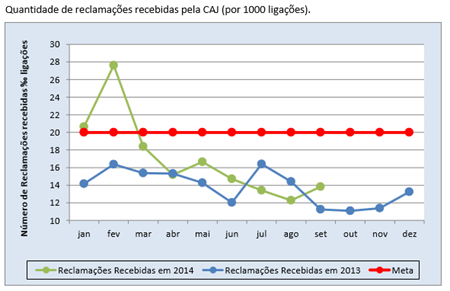
\includegraphics{figuras/LigacoesReclamacoes.png}
	\caption{Gráfico da Quantidade de Reclamações Mensais da CAJ}	
	Fonte - Companhia Águas de Joinville, 2014
\end{figure}


 Em 2013 o indicador de Número de Reclamações apresentou uma média anual de 13,78 reclamações/mil ligações de água, com uma quantidade notória de reclamações diárias se tornar custoso atender a todas solicitações individualmente utilizando somente atendentes sem que haja otimizações nos atendimentos, refletindo na média anual do tempo de espera das ligações para o \textit{Call Center} da companhia que no ano de 2013 que apresentou o tempo de 75,2 segundos por atendimento, deixando evidente o quão necessário se faz adotar medidas de melhorias nos sistemas de \textit{Call Center}. Conforme informações disponíveis no Sistema Nacional de Informações do Setor de Saneamento (SNIS) (SNIS, 2014), especificamente a Região Norte do país possui um dos piores índices de perda de faturamento do país, consequentemente isso gera lucros menores e ineficiência na ampliação do acesso à população aos serviços de saneamento, dificultando ainda mais investimentos por parte das companhias em tecnologias renovadores para o setor de saneamento. Visando propor soluções viáveis que possam agregar valor à empresa sem acarretar em custos elevados, utilizando de soluções em software \textit{Open Source} com tecnologias compatíveis, será possível tornar o próprio sistema principal de uma empresa de saneamento o GSAN, capaz de suprir através dos recursos da ferramenta Asterisk a necessidade em disponibilizar de forma prática e padronizada o acesso a informações geradas e mantidas pela empresa, consequentemente possibilidade de redução de custo com a utilização de uma unidade de resposta audível para realizar o atendimento de primeiro nível. Propiciando ao cliente final um melhor e mais efetivo relacionamento com a empresa prestadora de serviços.


\section{Aspectos de Inovação}
O trabalho de pesquisa e desenvolvimento se trata de uma integração entre software totalmente distintos, com tecnologia Open Source, onde juntos seram capazes de atender à uma demanda existente no setor de saneamento brasileiro relacionado ao contexto de Atendimento ao Público. Com a integração entre o sistema GSAN com o software Asterisk, será possível transferir os atendimentos destinado a central de atendimento, para uma Unidade de Resposta Audível (URA), executando a triagem das solicitações de forma padronizada e para solicitações referentes aos tipos de serviços Obter 2ª via de Conta, Informar Falta de Àgua e Solicitar Restabelecimento de Ligação, será possível realizar de forma automatizada o atendimento, sem que haja intervenção humana durante o processo. 
Não há oficialmente uma versão publicada na comunidade do sistema GSAN capaz de atender esta demanda de forma igual ou superior, inovando em propor uma solução viável e eficiente de baixo custo, para possibilitando a melhoria no atendimento ao cliente, se destacando em permitir que o cliente possa realizar suas solicitações em qualquer horário do dia ou noite, sem ter que se locomover a empresa e acessar informações de débitos pendentes de forma rápida e padronizada.

%\section*{Trabalhos Relacionados}
Este trabalho de pesquisa e desenvolvimento se assemelha ao trabalho descrito por Guilherme \cite{VIEIRA:2007}, que também utilizou recursos do programa Asterisk para desenvolver uma Sistema de criação de planos de discagem de forma prática explanando aspectos da ferramenta e expondo as dificuldades encontradas, apesar de ambos utilizarem dos diversos recursos do Asterisk, há divergência no objetivo onde este se destaca o fato de realizar uma integração com outro software, visando solucionar uma demanda do setor de Saneamento.

No trabalho desenvolvido por Jilcimaico \cite{DARU:2008}, aborda com clareza a utilização da distribuição Disc-OS como interface WEB do Asterisk, além de descrever os principais conceitos envolvidos na utilização do software, demonstra os procedimentos necessários para realizar a instalação da ferramenta e configuração dos recursos essências para um \textit{Call Center}, assemelhando-se este ao fato de também utilizar a distribuição Disc-OS que propõe uma interface WEB para a configuração do Asterisk.

O trabalho desenvolvimento por Humberto \cite{CAMPOS:2007}, utilizou os principais recursos do software Asterisk para realizar uma integração com um sistema externo que calcula os valores de cada ligação realizada, módulo chamado de “tarifador” além de exibir os valores em um hardware próprio, tal integração utilizou como referência tabelas em banco de dados para reconhecer eventos ocorridos e ações a serem tomadas, assemelhando-se a este trabalho pelo fato de utilizar recursos do Asterisk para disparar ações de sistemas externos, no entanto a forma de integração retratada acima se diferencia da forma adotada neste trabalho, que utiliza a interface AGI disponibilizada para comunicação com sistemas externos, o próprio Asterisk irá disparar ações a serem realizadas por meio de um \textit{Middleware} que implementa esta interface de comunicação.

Atualmente a empresa de saneamento Companhia Pernambucana de Saneamento \cite{COMPESA:URA} disponibilizou aos seus clientes o atendimento eletrônico por meio de URA, possibilitando a empresa realizar o atendimento destinado a central de atendimento, ou seja, o atendimento de primeiro nível, de forma automática e padronizada, propiciando também os direcionamentos entre ramais reais da empresa agilizando o atendimento e potencializando uma disponibilidade de 24 horas por 7 dias, com as informações à disposição dos clientes remotamente, porém a empresa não divulgou detalhes técnicos ou artefatos produzidos para realizar tal integração ou customização.
Para auxílio na elaboração deste trabalho de pesquisa se fez de grande valia os detalhes apontados sobre o \textit{software} Asterisk, principalmente a conceituação e protocolos disponibilizados para comunicação com sistemas externos, contidos no próprio \textit{website} da \textit{Digium \footnote{Disponível em: \url{http://www.digium.com/}}}. 

\section*{Método de Investigação}
A metodologia utilizada para realização do presente trabalho foi dívida da seguinte forma:
\begin{itemize}
	\item Pesquisa bibliográfica para obter o embasamento teórico sobre funcionamento dos sistemas envolvidos
	\item Identificação de uma possível forma de integração entre ambos;
	\item Desenvolvimento da integração entre os sistemas.
	\item Desenvolvimento de uma suíte de testes automatizados.
	\item Experimentação utilizando a suíte de testes automatizados
\end{itemize}

\section*{Estruturação da Monografia}
	
Após este capítulo introdutório, que basicamente visa contextualizar e caracterizar o tema de pesquisa, o trabalho realizado foi dividido em sete capítulos, conforme descrito abaixo:
\begin{description}
	\item \textbf{Capítulo 2} – Fundamentação Teórica – Este capítulo tem como objetivo abordar alguns dos conceitos do saneamento brasileiro e como o sistema GSAN está construído para atendê-lo, quais os módulos que compõem o sistema e detalhar a arquitetura do sistema, assim como expor os conceitos que envolvem o software Asterisk.
	\item \textbf{Capítulo 3 } – Revisão Bibliográfica – Será apresentado os principais conceitos utilizados como base no desenvolvimento deste trabalho.
	\item \textbf{Capítulo  4} – Processo de Integração – Trata-se da implementação realizada para integração entre os sistemas, apresentando as principais etapas para elaboração da comunicação entre os sistemas.
	\item \textbf{Capítulo  5} – Experimentação Utilizando a Suíte de testes Automatizados – Tem como característica a preparação do ambiente de teste, o planejamento e execução das experimentações utilizando a suíte de testes automatizados para validar a integração entre o sistema GSAN com o \textit{software} Asterisk.
	\item \textbf{Capítulo 6} – Conclusão – Neste capítulo, apresenta-se as conclusões que foram obtidas a partir deste trabalho.
	\item \textbf{Capítulo 7} – Considerações Finais e Trabalhos Futuros – Finalmente, no sétimo capítulo, apresentam-se recomendações para trabalhos futuros, reunindo os comentários finais deste trabalho de pesquisa.	
\end{description}
	

\section*{Cronograma}
A seguir será apresentado o cronograma com o planejamento mensal do início e termino das atividades previstas para conclusão do trabalho de pesquisa.

\begin{table}[htb]
	\center
	\footnotesize
	\begin{tabular}{|p{5cm}|p{0.8cm}|p{0.8cm}|p{0.8cm}|p{0.8cm}|p{0.8cm}|p{0.8cm}|p{0.8cm}|p{0.8cm}|}
		\hline
		\centering
		\textbf{Atividade} & \textbf{Jun} & \textbf{Jul} & \textbf{Ago} & \textbf{Set} & \textbf{Out} & \textbf{Nov} & \textbf{Dez}\\
		\hline
		Pesquisa bibliográfica. 			& \textbullet & \textbullet & - & - & - & - & - \\
		\hline
		Identificar formas de integração.	& - & \textbullet & \textbullet & - & - & - & - \\
		\hline
		Implementar a integração. 			& - & - & \textbullet & \textbullet & \textbullet & - & -  \\
		\hline
		Realizar experimentos. 				& - & - & - & - & \textbullet & \textbullet & - \\
		\hline
		Escrita da monografia. 				& \textbullet & \textbullet & \textbullet & \textbullet & \textbullet & \textbullet & \textbullet \\
		\hline
		Apresentação da monografia. 		& - & - & - & - & - & - & \textbullet \\		
		\hline
	\end{tabular}
\end{table}



% ----------------------------------------------------------
% PARTE I - Fundamentação
% ----------------------------------------------------------
%\part{Preparação da pesquisa}
\chapter[Fundamentação Teórica]{\textbf{F}undamentação \textbf{T}eórica}
%\addcontentsline{toc}{chapter}{Fundamentação Teórica}

\textit{Neste capítulo será apresentado o sistema GSAN e software Asterisk, com a intenção de familiarizar o leitor com as notações que serão amplamente utilizadas no decorrer do trabalho.}


\section{GSAN}
O sistema de código aberto GSAN\label{key:GSAN-TEORIA} (Sistema Integrado de Gestão de Serviços de Saneamento) desenvolvido inicialmente pela empresa IPAD (Instituto de Planejamento e Apoio ao Desenvolvimento Tecnológico e Científico) em 2005 por meio do Programa de Modernização do Ministério da Cidades, atualmente mantido e disponibilizado pelo Portal de Software Livre Brasileiro, sendo constantemente melhorado e aperfeiçoado pelos prestadores de serviços e interessados. 

Propõem-se em atender as principais demandas de gestão de operações comerciais e controle de execução de serviços nas companhias de saneamento do Brasil, que atualmente utilizam o sistema em grande escala, conforme exposto a seguir pela figura \ref{figura:implantacaoSistemaGSAN}:


\begin{figure}[H]
	\centering
	\caption{Implantações do Sistema GSAN}	
	\label{figura:implantacaoSistemaGSAN}
	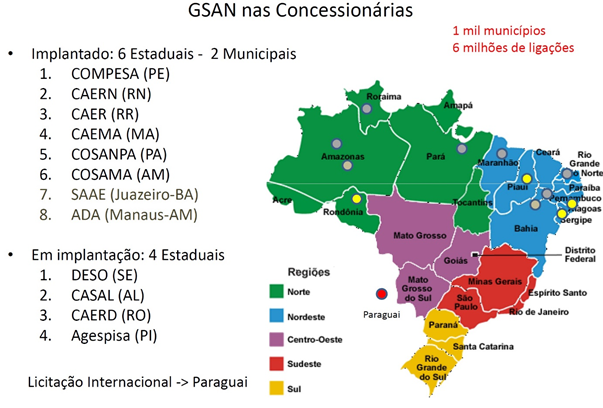
\includegraphics{figuras/implantacaoGSAN.png}
	\legend {\fontsize{10}{12}\selectfont {Fonte: \citeonline{PORTAL:2014}}.}
\end{figure}


Conforme demonstrado acima o sistema está em funcionamento em aproximadamente 1 mil municípios brasileiros, concentrado principalmente na região Norte e Nordeste do Brasil.
Atualmente o sistema está preparado para atender companhias de pequeno e médio porte, provendo soluções flexíveis através de parametrizações em tabelas de banco de dados, adequando-se a realidades distintas e tornando-se referência em software para o setor de saneamento básico brasileiro. 

\subsection{GSAN Conceitos}

O sistema em sua concepção foi dividido nos seguintes módulos descritos abaixo:
\begin{itemize}
\item \textbf{Atendimento ao Público}: Responsável principalmente em fornecer acesso rápido as informações dos clientes/imóveis e possibilita o registro dos atendimentos realizados.
\item \textbf{Cadastro}: Responsável em permitir a inserção, alteração e exclusão das entidades básicas só sistema.
\item \textbf{Micromedição}: Aborda as regras de consistência e análise de leitura e consumo, provendo meios para verificar o comportamento do consumo de água do imóvel.
\item \textbf{Faturamento}: Responsável principalmente em realizar o cálculo para precificar o consumo e gerar/emitir as faturas.
\item \textbf{Arrecadação}: Disponibiliza meios para efetuar a baixa de débitos dentre outras rotinas dessa natureza.
\item \textbf{Segurança}: Possibilita a gestão sobre as permissões de usuários/funcionários.
\item \textbf{Cobrança}: Fornece meios de emitir formas de cobranças personalizadas.
\item \textbf{Contabilização}: Realiza a contabilidade e possibilita integrações para sistemas externos.
\end{itemize}

Alguns dos conceitos de saneamento serão abordados neste trabalho, portanto faz-se necessário conhecer e entender como o sistema GSAN aborda essas questões.

O imóvel no sistema deve possuir relação com os seguintes itens (Tabela \ref{tabela:atributosImovel}):
\begin{table}[H]
	\center
	\footnotesize
	\caption{Principais Atributos do Imóvel}
	\label{tabela:atributosImovel}
	\begin{tabular}{|p{3cm}|p{7cm}|p{2.5cm}|} \hline
		\textbf{Atributo} 	& \textbf{Descrição}						& \textbf{Obrigatório}  \\ \hline
		Localidade 			& Um conjunto populacional					& Sim \\	\hline
		Setor Comercial 	& Conjunto de quadras, semelhante ao bairro & Sim \\ 	\hline
		Quadra 				& Denominado normalmente de "quarteirão" 	& Sim \\ 	\hline			
		Lote 				&  Uma subdivisão da Quadra 				& Sim \\ 	\hline
		Sub-Lote 			&  Uma subdivisão da Lote 					& Sim \\ 	\hline
	\end{tabular}
	\legend {\fontsize{10}{12}\selectfont {Fonte: Autoria Própria}.}
\end{table}


Tais relacionamentos são necessários para constituir a matrícula do imóvel, que forma um código único e representa a localização exata do imóvel.\\
\textbf{Matrícula:} [ Localidade ].[ Setor Comercial ].[ Quadra ].[ Lote ].[ Sub-Lote ]  \\
\textit{Ex: 001.015.080.0120.001}

O imóvel pode conter uma Ligação seja ela de Água, Poço e Esgoto, após o cliente realizar o cadastro do imóvel e solicitar a ligação, normalmente quando o imóvel obtém uma Ligação de Água ou Poço, é cobrado uma taxa mensal referente ao Esgoto variando em muito dos casos de 80\% a 100\% do valor a ser cobrado pelo consumo de água. Existem as possíveis situações para a Ligação do imóvel:
\begin{itemize}
	\item \textbf{Ligado}: Imóvel está conectado à rede de distribuição de água.
	\item \textbf{Potencial}: Imóvel está localizado fora do alcance da rede de distribuição de água.
	\item \textbf{Factível}: Imóvel está localizado dentro do alcance da rede de distribuição de água, mas que nunca esteve conectado a ela.
	\item \textbf{Cortado}: Imóvel que possui um dispositivo de vedação do fluxo de água no intuito de interromper o abastecimento.
	\item \textbf{Suprimido}: Imóvel que teve o ramal de água retirado para a interrupção definitiva do abastecimento de água.	
\end{itemize}

O relacionamento entre Clientes e Imóveis no sistema pode ocorrer das seguintes formas:
\begin{itemize}
	\item \textbf{USUÁRIO} – Pessoa que reside no imóvel.
	\item \textbf{PROPRIETÁRIO} – Pessoa que possui a propriedade do bem de direito.
	\item \textbf{RESPONSÁVEL} – Pessoa responsável pelo pagamento de débitos do imóvel.	
\end{itemize}

As solicitações realizadas pelos clientes aos atendentes são denominadas Registros de Atendimentos pelo sistema, comumente chamada de RA, para cada tipo de solicitação seja ela Solicitar Ligação, Solicitar Corte, Informar Falta de Água entre outras, o sistema possui tipos de serviços que devem ser realizados para atender à solicitação, a execução destes serviços é representado por uma  entidade denominada Ordem de Serviço, comumente chamada de OS, o sistema permite que seja configurada a criação de OS automáticas para determinadas solicitações, tornando menos burocrático a formalização das reclamações recebidas.


\subsection{GSAN Arquitetura}
	
O Sistema GSAN foi desenvolvido fundamentalmente utilizando a plataforma JEE\footnote{JEE - \textit{Java Enterprise Edition}}, propriedade da \textit{Oracle Corporation}, em sua versão 5, na época a mais recente. Utiliza os principais serviços e tecnologias oferecidos pela plataforma, como por exemplo, EJB\footnote{EJB - \textit{Enterprise Java Beans}}, JMS\footnote{JMS - \textit{Java Message Service}} e JSP\footnote{JSP - \textit{Java Server Pages}} 2.1.
O GSAN possui uma arquitetura que implementa diversos padrões de projeto, visando facilitar a manutenibilidade e manter a organização dos componentes, segue abaixo o diagrama de componentes conforme a figura \ref{figura:arquiteturaDetalhada}:

\begin{figure}[H]
	\centering
	\caption{Arquitetura Detalhada do Sistema GSAN}	
	\label{figura:arquiteturaDetalhada}
	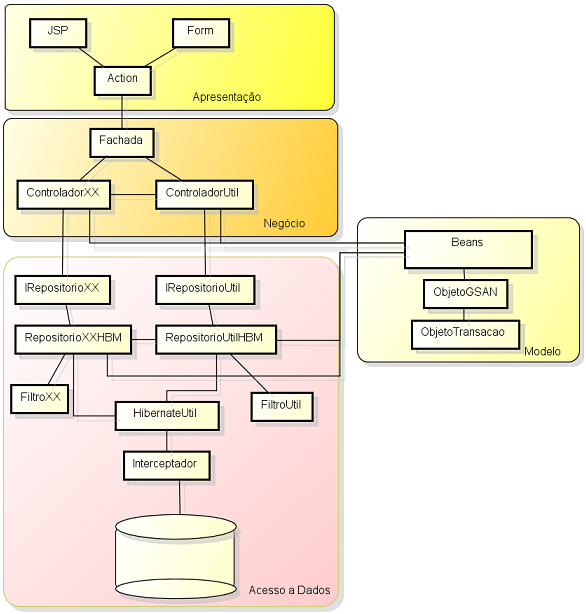
\includegraphics{figuras/gsanArquiteturaMenor.png}
	\legend {\fontsize{10}{12}\selectfont {Fonte: Autoria Própria}.}
\end{figure}

	
A camada de apresentação utiliza recurso nativo da plataforma JEE para Web, sendo a JSP para construção dos layouts e páginas a serem exibidas, juntamente com o \textit{framework} Apache Struts versão 1.2 atuando como controlador das requisições, além de Javascript e CSS para tratar o comportamento e aparência das páginas.
A fachada é um ponto de comunicação entre as camadas de apresentação e a camada de negócio e implementa o padrão de projeto \textit{Singleton}\footnote{\textit{Singleton} refere-se ao Padrão de Projeto que garante a existência de somente uma instância de determinada classe.}. 
A principal função da fachada é centralizar todas as chamadas de métodos da camada de negócio para que outras aplicações ou outras camadas superiores possam utilizar seus serviços.
As Classes de Controladores EJB são responsáveis por garantir toda a regra de negócio do sistema, elas são implementadas utilizando a especificação do \textit{Enterprise Java Beans} versão 2.1.
As classes de Repositório são classes da aplicação que utilizam o padrão de projeto \textit{Singleton}, a responsabilidade desta classe consiste em assegurar que todos os métodos de persistência ou serviço de consulta com o banco de dados.

O sistema GSAN foi projetado para ser independente da solução de Banco de Dados utilizada, acoplado ao \textit{framework} Hibernate que trata da persistência Objeto/Relacional (ORM), possibilita o isolamento da camada de Persistência.

A aplicação dos Padrões de Projetos renomados, tornar o código mais organizado e entendível, facilitando futuras manutenções, a utilização do padrão MVC\footnote{MVC - \textit{Model View Controller}} como estrutura arquitetural faz com que exista isolamento entre as camadas de Modelo, Visualização e Controle da aplicação, tornando a organização de pacotes bem estruturada.
	
	
\subsection{GSAN Configuração}
A configuração do ambiente de desenvolvimento se trata de um passo fundamental para execução deste trabalho prático. Primeiramente será preciso obter a versão do sistema que se encontra disponível no site do Portal do Software Livre, que atualmente disponibiliza o código fonte do sistema GSAN e demais arquivos de configuração do ambiente, no \textit{github}\footnote{Disponível em \url{http://www.github.com}} para a comunidade de desenvolvedores e interessados. 

Com o código fonte em mãos é necessário o auxílio de uma IDE\footnote{IDE - \textit{Integrated Development Environment}} de desenvolvimento para realizar a manutenção e construção dos novos serviços, foi utilizado neste trabalho a IDE Eclipse Juno para realizar esta tarefa, o processo de configuração da IDE pode ser visto descrito nos anexos deste trabalho.

O processo de empacotamento para geração do EAR (\textit{Enterprise Archive}) para disponibilização, utiliza a ferramenta Apache Ant versão 1.6.2, normalmente a versão disponibilizada pela comunidade possui \textit{script} de \textit{build}\footnote{\textit{Scripts} de \textit{build} refere-se a instruções para realizar o empacotamento da aplicação.} para serem executados, no entanto é preciso configurar os locais adequados para geração do pacote, conforme segue o exemplo abaixo na figura \ref{figura:configuracaoScriptBuild}:

\begin{figure}[H]
	\centering
	\caption{Exemplo de configuração do \textit{script} build}
	\label{figura:configuracaoScriptBuild}	
	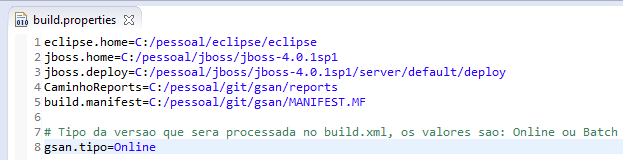
\includegraphics{figuras/build_properties.png}
	\legend {\fontsize{10}{12}\selectfont {Fonte: Autoria Própria}.}
\end{figure}
	
A execução do \textit{script} pode ser realizada dentro da IDE executando o seguinte procedimento, após localizar o arquivo \textit{build.xml} dentro na raiz do projeto, ao clicar com o botão esquerdo e selecionar a opção \textit{Run as > Ant Build}, será acionado a execução da instrução \textit{make} padrão do \textit{script}, para construção do pacote a ser disponibilizado, conforme visto na figura \ref{figura:execucaoScriptBuild}:	
		
\begin{figure}[H]
	\centering
	\caption{Execução do \textit{script} de build}
	\label{figura:execucaoScriptBuild}
	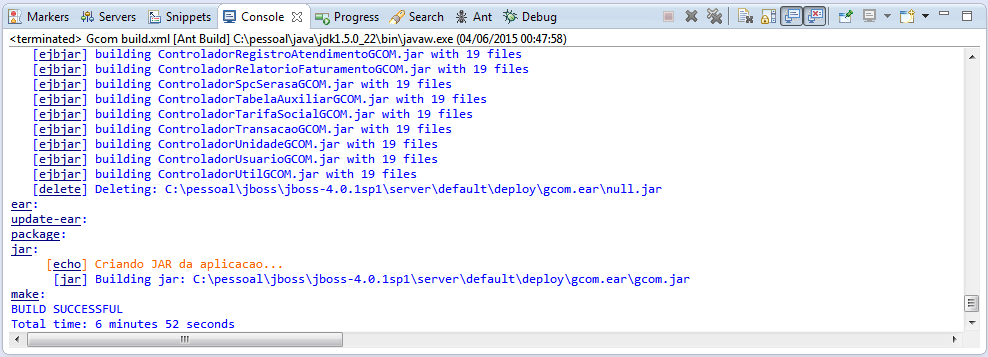
\includegraphics{figuras/build_ant.png}
	\legend {\fontsize{10}{12}\selectfont {Fonte: Autoria Própria}.}
\end{figure}

Para executar a aplicação faz-se necessário a utilização de um servidor de aplicação que implemente as principais interfaces de serviços da plataforma JEE que serão consumidos pela aplicação, neste trabalho foi utilizado o projeto \textit{Open Source Jboss Community} na versão 4.0.1, compatível com as tecnologias utilizadas no GSAN, a configuração deste Servidor de Aplicação Web pode ser consultado nos anexos deste trabalho.
Para executar o sistema GSAN, utilizando o terminal de comando do sistema operacional (\textit{Command Prompt}) basta digitar run e pressionar a tecla Enter será iniciado o servidor de aplicação e executará o sistema GSAN, visto na figura \ref{figura:execucaoSistemaGSAN}:


\begin{figure}[H]
	\centering
	\caption{Executando o sistema GSAN}	
	\label{figura:execucaoSistemaGSAN}
	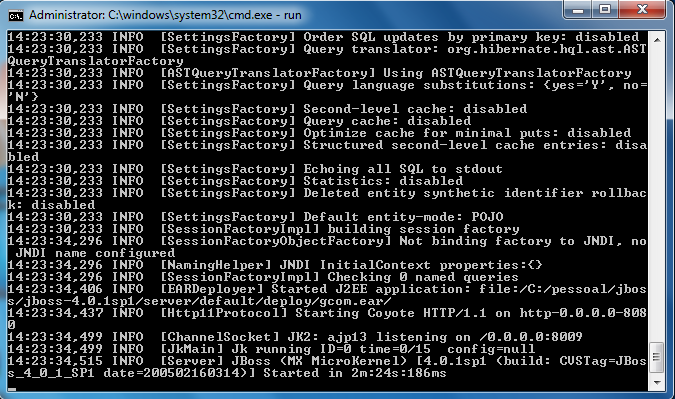
\includegraphics{figuras/executando_jboss.png}	
	\legend {\fontsize{10}{12}\selectfont {Fonte: Autoria Própria}.}
\end{figure}


A solução adotada para banco de dados neste trabalho será o PostgreSQL na versão 9.3.4 e PgAdmin versão 1.18.1 como SGBD (Sistema de Gerenciamento de Banco de Dados), no próprio site existe o guia de instalação para desenvolvedores tornando esse passo bem intuitivo.

Na versão do sistema GSAN disponibilizada para a comunidade, existe um diretório chamado \textbf{\textit{migrations}} que contém os \textit{scripts} de banco de dados necessários para criação das tabelas principais que o sistema exige para funcionar corretamente, e também disponibiliza todas instruções necessárias para a configuração dos datasources comercial e gerencial que serão utilizados no sistema GSAN.
Para acessar o sistema em execução, basta digitar o seguinte endereço no navegador http://127.0.0.1:8080/gsan, caso tudo ocorra bem deverá ser apresentada a página conforme visto na figura \ref{figura:acessoPaginaInicial} abaixo:

\begin{figure}[H]
	\centering
	\caption{Acessando página inicial do Sistema}
	\label{figura:acessoPaginaInicial}	
	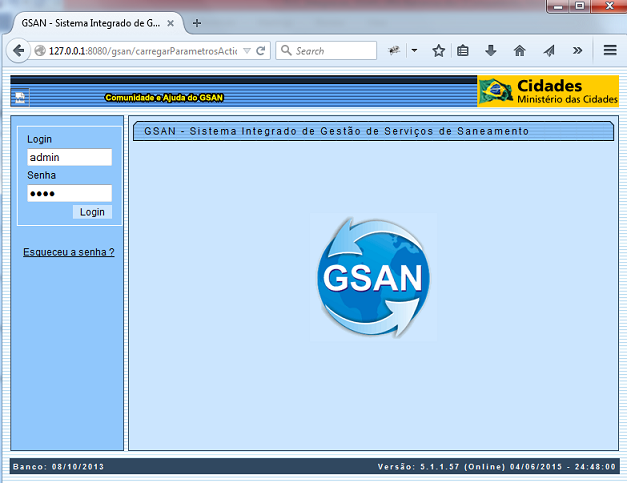
\includegraphics{figuras/gsan_online.png}	
	\legend {\fontsize{10}{12}\selectfont {Fonte: Autoria Própria}.}
\end{figure}


A credencial de acesso criada por padrão é: \\
\textbf{Login}: admin \\
\textbf{Senha}: gcom \\
Após inserir a credencial de acesso acima teremos acesso as todas as funcionalidades dos módulos do sistema GSAN.


\section{Asterisk}
A ferramenta de código aberto Asterisk desenvolvida pela Digium, disponibiliza as principais funcionalidades que um \textit{Call Center} necessita, dentre elas a criação de Ramais, Troncos, Rotas, configuração Plano de Discagens, Gravação de Voz, Conferência, Filas, Unidade de Resposta Audível entre diversos outros recursos que podem ser explorados e utilizados, podendo ser utilizado como um PABX IP, assim como se integrado a soluções VoIP ou a rede de telefonia publica.
Com tantos recursos disponíveis e sendo multiplataforma a ferramenta Asterisk está muito bem preparada para atender as expectativas, principalmente pelo fato de disponibilizar protocolos de comunicação com sistemas externos, por exemplo, o protocolo AGI (\textit{Asterisk Gateway Interface}), permite o consumo de recursos externos ao Asterisk, já o protocolo AMI (\textit{Asterisk Manager Interface}) permite que aplicações externas enviem ordens para serem executadas no Asterisk, dessa forma a solução pode ser muito bem integrada a sistemas legados.


\subsection{Asterisk Conceitos}

A ferramenta tem como base o Plano de Discagem, sendo ele responsável em definir o que deve acontecer, seja no momento em que for recepcionada uma ligação ou quando for digitado algum número. No plano de discagem podemos definir separações lógicas denominadas contextos, responsáveis em definir um comportamento utilizando os recursos nativos para determinar as instruções (extensões), por exemplo, podemos criar um contexto para definir o que deve acontecer ao receber ligações da rede pública e outro para definir o comportamento para as ligações advindas de ramais internos:

\begin{flushleft}

\textbf{[PSTN]} \\
\textit{exten => 2000,1,Answer();} \\
Contexto chamado “PSTN”, utiliza a extensão 2000, com prioridade 1 e aplicação Answer.\\

\textbf{[RAMAIS\_INTERNOS]} \\
exten => 2001,1, Playback(AVISO\_GERAL); \\
Contexto chamado “RAMAIS\_INTERNOS”, utiliza a extensão 2001, com prioridade 1 e aplicação Playback para tocar o áudio AVISO\_GERAL.\\
\end{flushleft}

O número 2000 no contexto “PSTN” utilizando na extensão representa o número informado pelo Originador da chamada, a prioridade trata-se de um parâmetro que representa a ordem de execução das aplicações, normalmente descritos de forma sequencial, já as aplicações são utilizadas para realizar uma ação qualquer. Em cada extensão (exten), podemos utilizar recursos de aplicativos nativos da ferramenta, sejam eles para atender, desligar, gravar o áudio entre outros recursos, dessa forma podemos definir o comportamento para o contexto, assim como realizar a transferência para outros contextos.


\subsection{Asterisk Instalação}

A instalação do Asterisk muita das vezes é uma tarefa cansativa e exige bastante atenção, pois a configuração deve ser realizada em arquivos de texto em uma sintaxe estabelecida pela ferramenta, atualmente existem diversas soluções que fornecem uma interface gráfica para tornar esse processo mais intuitivo e prático, neste trabalho foi utilizada uma distribuição chamada Disc-OS na versão 2.0, que disponibiliza uma interface web para realizar a configuração do Asterisk 1.4, para realizar o processo de instalação do Disc-OS, foram seguidos os passos descritos por Jilsimaico Darú (DARÚ, 2008), após a realização dos procedimentos, ao iniciar a distribuição Disc-OS automaticamente será iniciado o serviço do Asterisk, dessa forma para acessar o sistema basta digitar no navegador o endereço IP do terminal que está executando o sistema, visualizando a página conforme a figura 8 abaixo:


%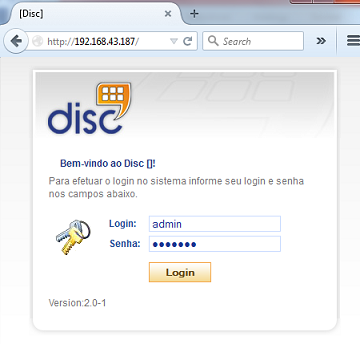
\includegraphics[scale=1]{figuras/pagina_inicial_asterisk}
\begin{center}
	IMAGEM PENDENTE \\
	Figura 8: Acessando página inicial da Interface WEB do Disc-OS \\
	Fonte: Autoria Própria \\
\end{center}

Para acessar as funcionalidades do sistema basta inserir a seguinte credencial de acesso:\\
\textbf{Login}: admin\\
\textbf{Senha}: disc-os\\


% Capitulo de revisão de literatura
\chapter[Revisão Bibliográfica]{\textbf{R}evisão \textbf{B}ibliográfica}
%\addcontentsline{toc}{chapter}{Revisão Bibliográfica}

\textit{Neste capítulo será apresentado o conceito dos \textit{frameworks} utilizados neste trabalho, além de justificar o motivo que levou a ser utilizados e destacar vantagens obtidas em seu uso.}


\section{Tecnologias Utilizadas}

No estudo para propor uma solução viável e consistente de integração entre sistemas, que seja realmente eficiente, é necessário entender todo o contexto em que está sendo operado o Sistema de Informação GSAN, visando identificar as informações mais relevantes acessadas pelo atendimento ao cliente, as principais dificuldades enfrentadas e os desafios que norteiam esse módulo do sistema. 


\subsection{GSAN - Detalhamento Técnico }

O GSAN por ser um sistema de informação adaptável a empresas de pequeno, médio e grande porte, contemplando soluções dos mais diversos requisitos, entre eles Cadastramento, Micromedição, Faturamento, Arrecadação, Cobrança, Negativação e Atendimento ao Cliente. Fornecendo de forma razoavelmente flexível as configurações e detalhes operacionais das rotinas, disponível em ambiente Web utilizando recursos de tecnologias software livre.

Para realização de melhorias no sistema GSAN faz-se necessário o ter conhecimento sobre os principais frameworks utilizados, a linguagem de programação utilizada e alguns conceitos de Saneamento que serão abordados.
Dos principais \textit{frameworks} utilizados, destaco o uso dos seguintes: \\

\textbf{Hibernate\footnote{Disponível em \url{http://www.hibernate.org}}}: Trata-se de um robusto framework de persistência de objetos relacionais, que fornece facilmente meios para realizar o mapeamento das entidades do sistema e diminui a complexidade de acesso a base de dados.\\

\textbf{Apache Struts\footnote{Disponível em \url{http://struts.apache.org/}}}: Tem como característica principal a sua utilização na construção de controladores utilizando o padrão \textit{Model View Control} (MVC) que se trata da separação das camadas utilizadas em uma aplicação, fornecendo uma maior organização no código fonte e contribui para futuras manutenções \cite{fowler2003}. 

O sistema GSAN faz uso da plataforma Java, lançado na versão Java Develop Kit (JDK) 1.5, utilizando recursos especificados pela \textit{Java Enterprise Edition} (JEE) \cite{PORTAL:2014}, essencialmente o container \textit{Enterprise Java Bean} (EJB), \textit{Java Server Pages }(JSP) e \textit{Servlets} que são executadas dentro de um servidor de aplicação Java EE.


\subsection{Asterisk - Detalhamento Técnico}
A ferramenta de código aberto Asterisk\footnote{Disponível em \url{http://www.asterisk.org}}, tem algumas características importantes e fundamentais para o estudo além de ser uma implementação de uma central telefônica que permite que clientes se comuniquem, tem outros recursos interessantes que fazem da ferramenta uma peça chave no processo da integração proposta, recursos como respostas interativas, correios de voz, realização de conferencias, distribuição automática de chamadas, além de ser flexível a adição de novos recursos tanto por meio de scripts na própria linguagem do Asterisk como também por meio de códigos em linguagem C entre outras formas de customização da ferramenta. Desenvolvido pela empresa Digium sob licença GPL (\textit{General Public Lisence}), atualmente portável em versões Linux, Windows e Mac OS, suportando protocolos de Voz sobre IP (VoIP), assim como SIP e H.323 entre outros. O próprio Asterisk contém um protocolo próprio chamado IAX fornecendo um melhor desempenho entre os entroncamentos entre os servidores Asterisk para casos de maior complexidade.

\subsection{Simple Object Access Protocol}
O protocolo SOAP\footnote{Disponível em  \url{http://www.w3.org/TR/soap}} (Simple Object Access Protocol) tem o objetivo de possibilitar a troca de informações estruturadas em Linguagem de Marcação Extensível (XML), para sistemas distribuídos. A negociação e transmissão de mensagens foram baseadas em outros em outros protocolos de serviços como o HTTP (Hypertext Transfer Protocol) e RPC (Remote Procedure Call), possibilitando a utilização para realizar integrações entre softwares.

\subsection{Asterisk Gateway Interface}
O software Asterisk possui uma interface de comunicação chamado AGI (\textit{Asterisk Gateway Interface}) \cite{asteriskAgi}, que tem como objetivo prover uma maior flexibilidade para adaptar soluções de linguagens diferentes, com esta interface se torna possível a comunicação com recursos externos através de requisição semelhantes ao CGI(\textit{Common Gateway Interface}) de servidores web, onde as requisições são originadas pelo próprio Asterisk, existem diversos \textit{frameworks} que implementam essa interface de comunicação, para este trabalho será utilizado o Asterisk-Java\footnote{Disponível em: \url{http://www.asterisk-java.org}}\label{key:asteriskjava}, por ser escrito em sob a plataforma Java e compatível com as tecnologias que foram utilizadas para a comunicação com o WebService do sistema GSAN.
O \textit{framework} Asterisk-Java possui diversos recursos disponíveis para comunicação com a ferramenta Asterisk, a seguir pode ser visto alguns dos principais propostos pelo framework;

\begin{itemize}
	\item Comunicação AGI - A classe BaseAgiScript.
	\item Comunicação HTTP - A classe ManagerConnection
	\item Ouvintes - As interfaces AsteriskServerListener e PropertyChangeListener.
	\item Controladores - A classes AsteriskServer e DefaultAsteriskServer
\end{itemize}


\subsection{WebServices}
O WebService\footnote{Disponível em \url{http://www.oracle.com/technetwork/java/javaee/tech/webservices-139501.html}} se trata de uma solução que permite que sistemas diferentes se comuniquem através requisições de protocolo HTTP a recursos identificados por um URI (\textit{Uniform Resource Identifier}) identifico a Web convencional, descritos e definidos usando XML (\textit{Extensible Markup Language}).

\subsection{Unidade de Resposta Audível}
A Unidade de Resposta Audível\label{key:URA} (URA) ou atendente eletrônico se trata de um software ou equipamento de \textit{Call Center}, que possibilita o atendimento das ligações de forma automática, tal solução traz como benefício à padronização dos atendimentos e tem potencial para automatização dos atendimentos, com inúmeras possibilidades de customização através de integrações com sistemas externo \cite{VIEIRA:2007}.

\subsection{Middleware}
O Middleware ou intermediário se trata de uma camada de software responsável em mediar à comunicação de outros sistemas, utilizado normalmente em ambientes que tendem a utilizar plataformas, linguagens ou protocolos de comunicação diferentes nas trocas de informação, sendo um dos recursos adotados neste trabalho, tal recurso descrito por \citeonline{ALMEIDA:2011}.

\subsection{Disc-OS}
O Disc-OS\footnote{Disponível em \url{http://sourceforge.net/projects/disc-os/}}\label{key:DISC-OS} refere-se a uma distribuição Linux (Cent-OS), customizada para utilização de PABX e PABX IP, abstrai toda a configuração de bibliotecas básicas e instalação do Asterisk (Disc-OS, 2015). Disponibiliza uma interface Web para configuração dos recursos, são algumas das vantagens, possuir disponível no idioma português brasileiro, além de tornar bem prático o processo de configurações.

\subsection{Codec}
O codec (COder/DEcoder) se trata de processo de codificação e decodificação da voz humana a ser transmitidas entre a origem e destino em meio digital \cite{VIEIRA:2007}.

\subsection{JUnit Framework}
O JUnit framework\footnote{Disponível em \url{http://junit.org/}} destina-se a garantia da qualidade do software, viabilizando a construção dos mais diversos tipos de testes através 
do seu arcabouço de recursos disponíveis, por ser software livre e adotado como padrão nas principais IDE de desenvolvimento Java, ganhou grande popularidade nas comunidades de desenvolvedores. O desenvolvimento de testes unitários tem sido adotado como métricas de qualidade na entrega do produto de software.
O \textit{framework} tornou a escrita de testes um processo fácil e intuitivo, fazendo uso de recurso da plataforma Java chamado \textit{Annotation}\label{key:annotation}, trouxe a possibilidade de padronizar os métodos de testes apenas adicionando anotações sobres os mesmo, segue abaixo algumas anotações comumente utilizadas;

\begin{itemize}
	\item @Test - Anotação que representa um método de teste.
	\item @Before - Anotação indica que o método anotado será executado sempre antes de um método de teste.
 	\item @After - Anotação indica que o método anotado será executado sempre após a um método de teste.
\end{itemize}

O JUnit possui um objeto chamado \textit{Assert}, que contém uma série de validações possíveis para checagem do resultado esperado pelo teste.



% ----------------------------------------------------------
% PARTE II - CORE
% ----------------------------------------------------------
% INTEGRAÇÃO
\chapter[Processo de Integração]{\textbf{P}rocesso de \textbf{I}ntegração}
\addcontentsline{toc}{chapter}{Processo de Integração}

\textit{Neste capítulo são apresentados os procedimentos para a integração dos sistemas envolvidos, expondo o detalhes de implementação e configuração da solução proposta.}


\section{Definição da Solução}

Após o estudo aprofundado sobre o sistema GSAN e software Asterisk foram identificadas diversas formas de realizar a integração, entre os sistemas pelo fato da existência de várias protocolos possíveis de comunicação , no entanto a solução adotada será visando a reusabilidade, baixo custo de manutenção e o uso de tecnologias que já tenham uma maturidade no mercado. Foram escolhidos os protocolos SOAP e AGI para serem implementados por um \textit{Middleware}, este será responsável em assumir o papel de intermediário entre os sistemas GSAN e Asterisk. Com o intuito de facilitar o entendimento da comunicação entre os sistemas, a seguir será exposto o diagrama de implantação da solução (figura 9) descrita acima, explanado os principais detalhes adotados nesta integração:

\begin{figure}[!htb]
	\centering
	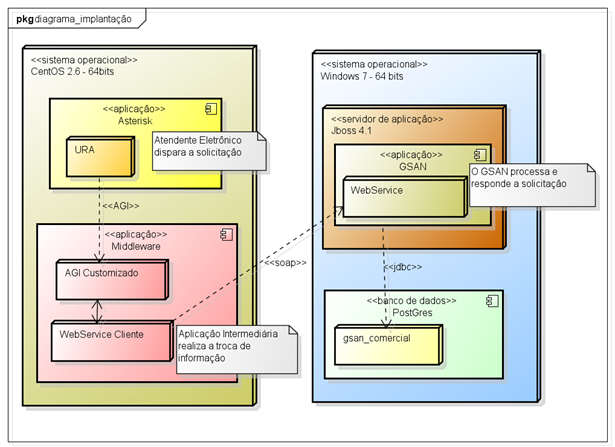
\includegraphics{figuras/diagrama_implantacao.png}
	\caption{Diagrama de implantação da solução}	
	Fonte - Autoria Própria
\end{figure}


Conforme ilustrado acima, o sistema GSAN irá prover uma interface de serviços na forma de WebServices utilizando o protocolo de comunicação SOAP (\textit{Simple Object Access Protocol}), tais serviços serão consumidos através do \textit{Middleware} intermediário denominado integrador que além de consumir os serviços do sistema GSAN, deverá também prover uma interface de serviços na forma utilizando o protocolo AGI, para então ser consumidos pelo Asterisk e responder a solicitação da Unidade de Resposta Audível.


\section{Tecnologias Utilizadas}
O processo de integração será composto por tecnologias com paradigmas diferenciados, no entanto para melhorar o entendimento dos detalhes de compatibilidades adotados segue abaixo a tabela 3 das tecnologias utilizadas e versões correspondentes.


\begin{table}[htb]
	\center
	\footnotesize
	\begin{tabular}{|p{4cm}|p{7cm}|p{2cm}|}
		\hline
		\textbf{Software} & \textbf{Finalidade} & \textbf{Versão} \\
		\hline
		Java Platform, \textit{Enterprise Edition} 5 (JEE) & Conjunto de Tecnologias e Serviços para implementar soluções da Plataforma Java com estabilidade, segurança e escalabilidade. & 5 \\
		\hline
		JBoss & Servidor de aplicação que implementa especificações JEE. & 4.0.1 sp1 \\
		\hline
		Hibernate & Framework utilizado para fazer o mapeamento objeto-relacional. É responsável pela camada de persistência. & 3.1 \\
		\hline
		PostgreSQL & Banco de dados relacional. & 9.3.4 \\
		\hline
		Apache Ant & Geração de \textit{Enterprise Application Resources} (EAR) deploy’s. & 1.6.2 \\
		\hline
		JasperReports & Tecnologia utilizada para criação de relatórios em PDF, HTML, XLS, CSV e XM.L & 1.2.2 \\
		\hline
		Struts & Framework para controle de navegação e validação Web. & 1.1	 \\
		\hline
		Disc-OS & Distribuição CentOS 2.6 que implementa interface web para a ferramenta Asterisk. & 2.0-1 \\
		\hline
		Asterisk & Software livre que permite a criação de PABX com diversos recursos. & 1.4 \\		
		\hline
		Asterisk-Java & Framework para comunicação com o Asterisk via protocolo AGI. & 1.0 \\				
	\end{tabular}
\end{table}

\begin{center}
	Tabela 3: Tecnologias utilizadas 
	Fonte: Autoria Própria
\end{center}


\section{Etapas da Integração}
O processo de integração entre os sistemas será composto por três etapas principais, das quais serão necessários para compor a solução escolhida, conforme definido abaixo e descrito nas sessões seguintes:

\begin{itemize}
	\item Implementar WebServices no Sistema GSAN 
	\item Desenvolver Middleware
	\item Customizar o Asterisk	
\end{itemize}

\subsection{\fontsize{12}{1} \selectfont{\textbf{Implementação de Webservices no GSAN}}}

A estratégia de desenvolver o Webservice internamente ao sistema GSAN, foi adotada visando a possibilidade de reaproveitamento das regras de negócio, entidade, controlados dentre os demais artefatos que fazem parte do sistema.  Os novos serviços foram desenvolvidos sob tecnologias compatíveis com as utilizadas no sistema GSAN, utilizando a especificação JAX-WS\footnote{JAX-WS - \textit{Java API for XML-Based Web Services}}  para serem consumidos por sistemas externos através de submissões de arquivos do tipo XML, definidas no padrão de comunicação SOAP. Para tratar de conversões de arquivos XML para objetos e vice-versa está sendo utilizada a especificação do padrão JAXB\footnote{JAXB - \textit{Java Architecture for XML Binding}}, dessa forma estes serviços são executados no mesmo servidor de aplicação.
Na prática é necessário importar ao projeto as seguintes bibliotecas descritas abaixo;

% LIBS UTILIZADAS
 Prover suporte a configuração do End-Points (Serviços);
	\begin{itemize}
		\item jaxws-api-2.2.jar
		\item jaxws-rt.jar
		\item jaxws-tools.jar		
	\end{itemize}
	Fornecer suporte ao tratamento de serialização\footnote{Serialização refere-se ao processo de conversão de um objeto em bytes.} dos XML;
	\begin{itemize}
		\item jaxb-impl.jar
		\item jaxb-xjc.jar
		\item policy.jar
		\item stax-ex.jar
		\item stax2-api.jar
		\item streambuffer.jar
		\item woodstox-core-asl.jar		
	\end{itemize}


Após realizar a configuração das bibliotecas necessárias para implementação, foram definidos os seguintes novos serviços para automatizar os processos de Obtenção da 2ª via de conta, Informar Falta de Água e Solicitar Restabelecimento da Ligação;

\begin{description}
	\item \textbf{\textit{isOnline}}: Realiza verificação de disponibilidade do sistema.
	\item \textbf{\textit{pesquisarImovelOuCliente}}: Obtém detalhes sobre um imóvel ou cliente cadastro no sistema GSAN.
	\item \textbf{\textit{obter2ViaConta}}: Gerar a 2ª via de conta pendente.
	\item \textbf{\textit{informarFaltaAgua}}: Formalizar junto ao sistema GSAN um Registro de Atendimento do tipo Falta de Água.
	\item \textbf{\textit{solicitarRestabelecimento}}: Formalizar junto ao sistema GSAN um Registro de Atendimento do tipo Solicitar Restabelecimento da Ligação de Água.
\end{description}

A figura \ref{figura:interfaceServicosAutomatizados} abaixo, demonstra a declaração dos métodos do \textit{Webservice}.

\begin{figure}[H]
	\centering
	\caption{\textbf{Interface dos serviços automatizados.}}	
	\label{figura:interfaceServicosAutomatizados}
	\begin{subfigure}[H]{\textwidth}
		\centering
		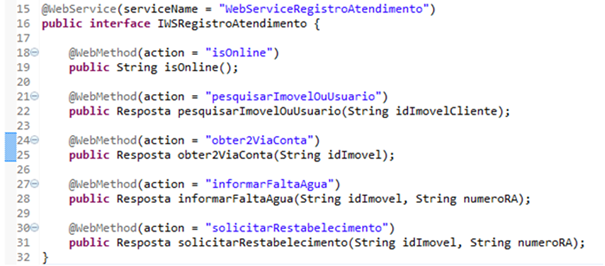
\includegraphics{figuras/implementacao_servicos.png}
		\legend {\fontsize{10}{12}\selectfont {Fonte: Autoria Própria}.}	
	\end{subfigure}
\end{figure}



Para definir a URL\footnote{URL - \textit{Uniform Resource Locator}} de acesso ao \textit{Webservice} será preciso atualizar o arquivo web.xml, declarando a servlet padrão definida na especificação do JAX-WS para esse propósito, conforme a figura \ref{figura:declaracaoServlet}:

\begin{figure}[H]
	\centering
	\caption{\textbf{Declaração da servlet do Webservice.}}	
	\label{figura:declaracaoServlet}
	\begin{subfigure}[H]{\textwidth}
		\centering
		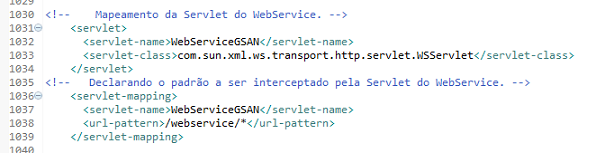
\includegraphics{figuras/declarando_servlet.png}
		\legend {\fontsize{10}{12}\selectfont {Fonte: Autoria Própria}.}	
	\end{subfigure}
\end{figure}

Feito isso, será preciso disponibilizar os novos serviços, definindo a Classe Concreta\footnote{Classe Concreta refere-se a classes que possuem atributos, métodos e construtores, passível de instanciação.} de implementação e o padrão de acesso que será adotado para a interface criada, para que as solicitações sejam interceptadas adequadamente redirecionadas ao \textit{EndPoints} corretos, com isso será necessário criar o arquivo com a seguinte nomenclatura \textit{sun-jaxws.xml}, localizado dentro do diretório WEB\_INF da aplicação, segue abaixo o conteúdo do arquivo, conforme a figura \ref{figura:declaracaoEndPoint}:

\begin{figure}[H]
	\centering
	\caption{\textbf{Declaração do \textit{EndPoint} dos serviços.}}	
	\label{figura:declaracaoEndPoint}
	\begin{subfigure}[H]{\textwidth}
		\centering
		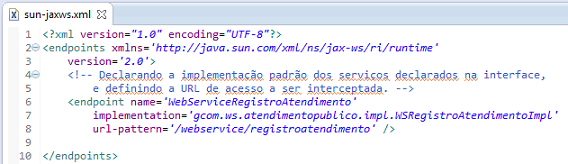
\includegraphics{figuras/declaracao_endpoint.png}
		\legend {\fontsize{10}{12}\selectfont {Fonte: Autoria Própria}.}
	\end{subfigure}
\end{figure}


Realizado todos esses passos o sistema GSAN conseguirá disponibilizar os novos serviços declarados na interface de Registro de Atendimento, dessa forma o acesso será realizado da seguinte maneira:

\begin{description}
	\item htttp://<servidor>:<porta>/gsan/webservice/registroatendimento
\end{description}

Estando apto a ser integrado com sistemas externos. 
\subsection{\textbf{\uppercase{Implementação do Middleware}}}

O \textit{Middleware} intermediário denominado Integrador será responsável em receber as solicitações realizadas pela URA do Asterisk, após analisá-las deverá efetuar requisições ao \textit{WebService} do sistema GSAN, a fim de obter as informações, logo em seguida tratá-las e então devolver as informações essenciais ao Asterisk.
O \textit{Middleware} é capaz de comunicar-se com os sistemas GSAN e Asterisk. A comunicação com o sistema GSAN é realizada por uma implementação cliente do \textit{Webservice} disponibilizado, já a comunicação com o Asterisk é realizada por uma interface de comunicação chamada AGI, neste trabalho foi utilizado o \textit{framework} \textit{Open Source} chamado Asterisk-Java, que fornece recursos para comunicação com o Asterisk utilizando os protocolos comuns ao sistema.

Para cada novo serviço a ser tratado pelo Middleware, é necessário declarar uma chave de texto que será utilizada no Asterisk, que representa o objeto a ser invocado, adicionados em um novo arquivo chamado \textit{fastagi-mapping.properties} da seguinte maneira, conforme a figura \ref{figura:mapeamenteServicosAGI} abaixo:

\begin{figure}[H]
	\centering
	\caption{\textbf{Mapeamento dos serviços para consumo via AGI}}
	\label{figura:mapeamenteServicosAGI}
	\begin{subfigure}[H]{\textwidth}
		\centering
		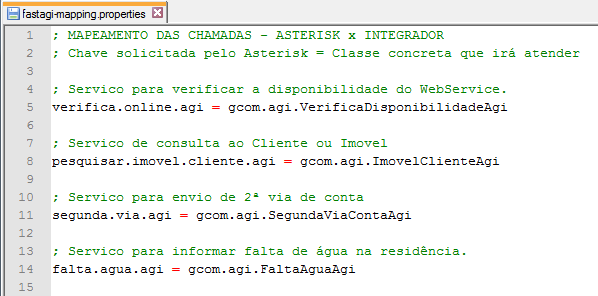
\includegraphics{figuras/mapeamento_servicos_agi.png}
		\legend {\fontsize{10}{12}\selectfont {Fonte: Autoria Própria}.}	
	\end{subfigure}
\end{figure}



Dessa forma o \textit{Middleware} tem condições de recepcionar as solicitações originadas pelo \textit{software} Asterisk utilizando a interface de comunicação AGI, e direcionar a chamada internamente para uma classe concreta que contém a lógica de consumo aos novos serviços disponibilizados pelo \textit{WebService} do sistema GSAN.

Para cada classe concreta a ser disponibilizada é necessário estender a classe \textit{BaseAgiScript} disponibilizada pelo \textit{framework} Asterisk-Java, em seguida é preciso implementar o método \textit{service} obtido pela herança da \textit{BaseAgiScript}, tal método será invocado quando a requisição for direcionada ao serviço mapeado no arquivo \textit{fastagi-mapping.properties}, segue abaixo um exemplo de implementação utilizado, conforme a figura \ref{figura:fluxoIdentificacaoClienteAsterisk} abaixo:

% Custom exibição da lista de algoritmos
%\algsetup{
%	linenosize=\small,
%	linenodelimiter=.	
%}

%\begin{algorithm}
%	\caption{Novo serviço de identificação do cliente (\textit{Middleware}).}	
%	\label{algoritmo:identificaoCliente}
%	\begin{algorithmic}[1]
%		\STATE $atenderLigação()$ 		
%		\COMMENT{Recepciona a liga}
%		\STATE $digitoInformado \gets canal[cliente]$ 	\COMMENT{Obtém os dígitos informados}
%		\IF{ $valorInformado <> null$ }
%		\STATE $ws \gets obterWebService() $ 
%		\COMMENT{Obtém a instância do WebService}
%		\STATE $retorno \gets ws.pesquisarImovelOuCliente(valorInformado) $
%		\COMMENT{Realiza a requisição}
%		\STATE $ tratarRetorno(retorno) $
%		\COMMENT{Verifica o retorno obtido}
%		\ELSE		
%		\STATE $ tocarAudio(informar\_valor) $
%		\COMMENT{Tocar o áudio de aviso}
%		\STATE $ canal[situacao] \leftarrow erro $
%		\COMMENT{Sinaliza o erro}
%		\ENDIF		
%	\end{algorithmic}
%\end{algorithm}

\begin{figure}[H]
	%\centering
	\caption{\textbf{Fluxo de Identificação de Cliente no Asterisk.}}	
	\label{figura:fluxoIdentificacaoClienteAsterisk}
	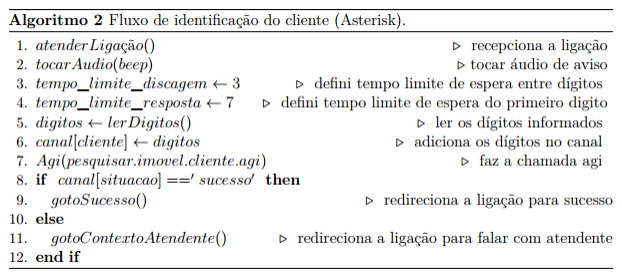
\includegraphics{figuras/algoritmo_2.png}
	\\[6pt]
	\fontsize{10}{12}\selectfont {Fonte: Autoria Própria.}

\end{figure}
%	\legend{\fontsize{10}{12}\selectfont {Fonte: Autoria Própria.}}

Visando facilitar o consumo dos novos serviços, será gerado o \textit{WebService} cliente a partir do WSDL\footnote{WSDL - \textit{Web Services Description Language}} da interface do serviço disponibilizada no sistema GSAN, utilizando o software chamado WSIMPORT disponibilizado pela \textit{Sun Microsystems}, conforme visto na figura \ref{figura:gerarWSCliente}:

\begin{figure}[H]
	\centering
	\caption{\textbf{Geração do código fonte para consumo do WebService.}}	
	\label{figura:gerarWSCliente}
	\begin{subfigure}[H]{\textwidth}
		\centering
		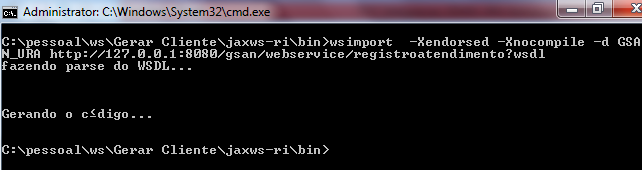
\includegraphics{figuras/gerar_wscliente.png}
		\legend {\fontsize{10}{12}\selectfont {Fonte: Autoria Própria}.}	
	\end{subfigure}
\end{figure}

Descrição dos parâmetros utilizados:

\begin{description}
	\item \textbf{\textit{–Xendorsed}}: Necessário para realizar a substituição dos padrões endossados do sistema, ou seja, utiliza a versão correta da JDK para realizar o \textit{parser}.
	\item \textbf{\textit{–Xnocompile}}: Utilizado para gerar o código fonte não compilado, ou seja, o arquivo na extensão .java.
	\item \textbf{\textit{-d}}: Informado para determinar o diretório para onde os arquivos devem ser gerados, no exemplo o diretório se chama "GSAN\_URA".
	\item Por último a URL que disponibiliza o WSDL dos serviços. 
\end{description}



Com isso será gerado o código fonte de consumo dos serviços atualmente declarados na interface do \textit{EndPoint}, para cada modificação na interface será necessário realizar o procedimento novamente. O \textit{Middleware} deve ser disponibilizado em um terminal, que seja acessível ao Asterisk, para que o mesmo consiga realizar requisições aos objetos mapeados anteriormente, neste trabalho o \textit{Middleware} foi executado no mesmo hospedeiro do Asterisk, conforme visto na figura \ref{figura:executarIntegrador} abaixo:

\begin{figure}[H]
	\centering
	\caption{\textbf{Executando o sistema Integrador.}}	
	\label{figura:executarIntegrador}
	\begin{subfigure}[H]{\textwidth}
		\centering
		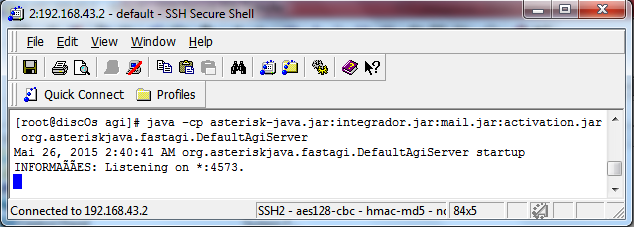
\includegraphics{figuras/executar_integrador.png}
		\legend {\fontsize{10}{12}\selectfont {Fonte: Autoria Própria}.}	
	\end{subfigure}
\end{figure}


A instrução realizada acima executa a classe principal do \textit{framework} Asterisk-Java a \textit{ org.asteriskjava.fastagi.DefaultAgiServer}, inicializando o serviço de comunicação via AGI, sob a JVM\footnote{JVM - \textit{Java Virtual Machine}} da plataforma Java, passando como \textit{Classpath}\footnote{Classpath refere-se a uma variável de ambiente que indica o local onde as dependências estão localizadas.} as seguintes bibliotecas: 
%Citar classpath - pendente

\begin{itemize}
	\item \textbf{\textit{asterisk-java.jar}}: biblioteca do \textit{framework} utilizado para se comunicar com o Asterisk.
	\item \textbf{\textit{integrador.jar}}: o \textit{Middleware} que integra as aplicações.
	\item \textbf{\textit{mail.jar}} e \textbf{\textit{activation.jar}}: ambos necessários no envio de e-mail, para os casos de Obter 2ª via de conta.	
\end{itemize}

Após estes passos o sistema Integrador já estará apto a receber solicitações do Asterisk e realizar requisições para o Sistema GSAN.
\subsection{Customizar o Asterisk}

A customização do Asterisk será fundamental para realizar a comunicação entre os sistemas, sendo responsável em disponibilizar de forma padronizada o acesso a URA no atendimento de primeiro nível de todas as chamadas recebidas, e disparar solicitações a recursos externos conforme a necessidade do cliente que efetuou a ligação.
Primeiramente iremos configurar um ramal, utilizando a interface web do Disc-OS, conforme exemplo abaixo na figura \ref{figura:cadastroRamapSIP}:


\begin{figure}[H]
	\centering
	\caption{Cadastro de um Ramal SIP.}	
	\label{figura:cadastroRamapSIP}
	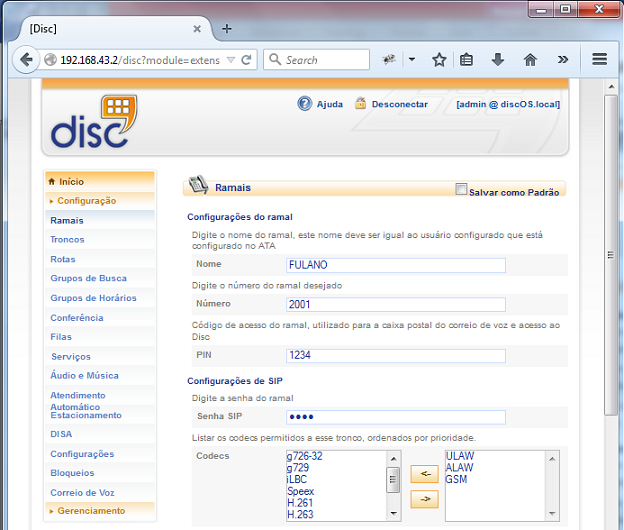
\includegraphics{figuras/cadastro_ramal_sip.png}
	\legend {\fontsize{10}{12}\selectfont {Fonte: Autoria Própria}.}
\end{figure}


Conforme visto acima, está sendo configurado o ramal de número 2001, com o nome de FULANO e definido alguns \textit{codecs} que serão permitidos utilizar neste ramal, após isto o Disc-OS se encarregará de alterar o arquivo de propriedades \textit{sip.conf} inserindo o ramal desejado com as características informadas.
Para a configuração da Unidade de Resposta Audível, será preciso definir claramente quais serão as opções disponíveis e quais serão as possíveis saídas com o seus devidos tratamentos, neste trabalho foi desenvolvido um fluxo de atendimento próprio, demonstrado na figura \ref{figura:fluxoURA}: 

\begin{figure}[H]
	\centering
	\caption{Diagrama do Fluxo da Unidade de Resposta Audível}
	\label{figura:fluxoURA}	
	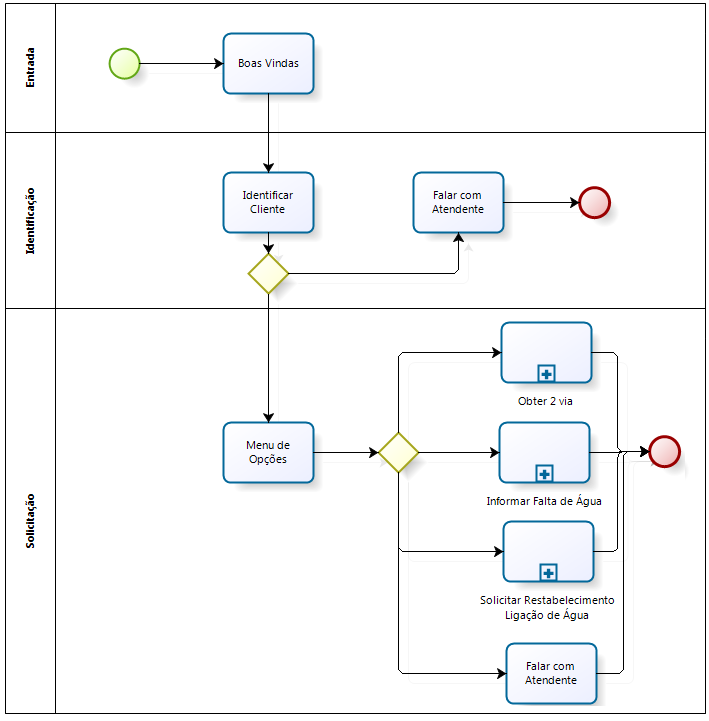
\includegraphics{figuras/fluxo_ura.png}
	\legend {\fontsize{10}{12}\selectfont {Fonte: Autoria Própria}.}
\end{figure}


Dessa forma o cliente terá a opção de falar com o atendente logo no primeiro menu de atendimento e nos demais sub fluxos, comportamento exigido conforme o artigo 4 da Lei nº 8.078 \cite{leiAtendimentoAoConsumidor}, que fixa normas gerais sobre o Serviço de Atendimento ao Consumidor, após realizar o passo de identificação o mesmo terá acesso as opções de serviços automatizados via integração caso ocorra tudo com êxito, caso não seja possível identificar o cliente será redirecionado para o Falar com Atendente.
A interface \textit{Web} do Disc-OS permite realizar a configuração da URA, de forma bem intuitiva, inclusive definir tempos de espera, direcionamento para outros Ramais entre outras configurações que tornam o processo de configuração muito mais prático, no entanto para configurar o fluxo da URA realizando a comunicação via AGI com o \textit{Middleware} será preciso realizar o procedimento manual de configuração, segue abaixo a configuração utilizada para criação do contexto de PESQUISAR\_CLIENTE utilizada para identificar o cliente, descrito no arquivo \textit{/etc/asterisk/extensions.conf}, conforme representado pelo algoritmo \ref{algoritmo:FluxoIdentificaoCliente} abaixo:


% Custom exibição da lista de algoritmos
\algsetup{
	linenosize=\small,
	linenodelimiter=.	
}

\begin{algorithm}
	\caption{Fluxo de identificação do cliente (Asterisk).}	
	\label{algoritmo:FluxoIdentificaoCliente}
	\begin{algorithmic}[1]
		\STATE $atenderLigação()$ \COMMENT{ recepciona a ligação}
		\STATE $tocarAudio(beep)$   \COMMENT{tocar áudio de aviso}
		\STATE $tempo\_limite\_discagem \gets 3$  \COMMENT{ defini tempo limite de espera entre dígitos }		 
		\STATE $tempo\_limite\_resposta \gets 7$  \COMMENT{ defini tempo limite de espera do primeiro digito}
		\STATE $digitos  \gets lerDigitos()$  \COMMENT{ ler os dígitos informados }
		\STATE $canal [cliente]  \gets digitos$   \COMMENT{ adiciona os dígitos no canal  }
		\STATE $Agi(pesquisar.imovel.cliente.agi)$  \COMMENT{ faz a chamada agi }
		\IF { $canal [situacao] == 'sucesso'$ }
		\STATE $gotoSucesso()$  \COMMENT{ redireciona a ligação para sucesso }
		\ELSE
		\STATE $ gotoContextoAtendente()$  \COMMENT{ redireciona a ligação para falar com atendente	}
		\ENDIF		
	\end{algorithmic}
\end{algorithm}


Neste trecho é declarado o contexto [PESQUISAR\_CLIENTE], cuja prioridade 1 será anteder a ligação e logo em seguida emitir um áudio chamado \textit{"beep"}, foi defini o tempo limite de espera para o primeiro dígito de 7 segundos e o tempo limite de espera para a discagem dos dígitos de 3 segundos, será lido os valores informados pelo Originador da chamada e atribuída a variável CLIENTE\_IMOVEL, após isto será realizada uma requisição via interface de comunicação  AGI para o \textit{Middleware}, solicitando o serviço mapeando em pesquisar.imovel.cliente.agi, dependendo do retorno deste serviço será realizado um redirecionamento da ligação para um contexto específico, para consultar a configuração completa da URA encontra-se disponível nos anexos deste trabalho.
Para tanto, será necessário customizar os arquivos de áudio para serem tocados, conforme as operações disponíveis forem acessadas. Para efetuar a gravação do áudio foi utilizado um recurso do Asterisk, discando para *77, existe um contexto que utiliza aplicativos nativos para realiza a gravação no formato WAV e o disponibiliza no diretório \textit{/var/lib/asterisk/sounds/custom/} para utilização.
Após as configurações básicas, será preciso ter um dispositivo para efetuar as chamadas e conseguir se comunicar com a URA, neste cenário existe um recurso chamado de \textit{Softphone}, são programas que tornam o computador em um Ramal IP, possibilitando realizar e receber chamadas, com essa finalidade foi utilizado o Zoiper\footnote{Disponível em \url{https://www.zoiper.com/}}, conforme visto na figura \ref{figura:zoiper}:

\begin{figure}[H]
	\centering
	\caption{Softphone Zoiper sendo executado}	
	\label{figura:zoiper}
	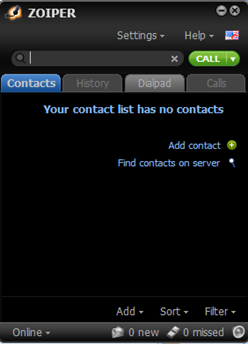
\includegraphics{figuras/zoiper.png}
	\legend {\fontsize{10}{12}\selectfont {Fonte: Autoria Própria}.}
\end{figure}


Para adicionar o ramal é preciso definir qual será o protocolo utilizado e inserir os dados configurados no Asterisk conforme visto na figura \ref{figura:zoiperConfigRamal} abaixo:

\begin{figure}[H]
	\centering
	\caption{Configurar Ramal no Zoiper}
	\label{figura:zoiperConfigRamal}
	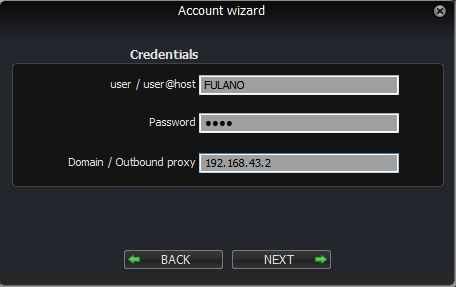
\includegraphics{figuras/configurar_ramal_zoiper.png}
	\legend {\fontsize{10}{12}\selectfont {Fonte: Autoria Própria}.}
\end{figure}

Após realizar todos estes passos será possível acessar os serviços disponibilizados pela URA, através do Zoiper efetuar as chamadas para percorrer os fluxos previamente definidos.
\subsection{Desenvolver Suíte de Testes Automatizados}

A suíte de testes automatizados será responsável em garantir o correto funcionamento da integração entre os sistemas envolvidos, ou seja prover um meio onde possa ser testado tanto o Webservice do GSAN quanto a \textit{interface} Agi implementada para o Asterisk, para essa situação foram utilizados recursos do JUnit para criação dos cenários de teste, execução dos testes e identificação de falhas, quanto recursos do \textit{framework} Asterisk-Java para simular e controlar chamadas telefônicas com parametrização dinâmica.   

Cada classe de teste deve implementar uma interface do framework Asterisk-Java chamada \textit{PropertyChangeListener} e posteriormente ser registrada como \textit{Listener} em uma classe da suíte chamada \textit{SuiteAsteriskListener}, que atua como uma escuta de modificações ocorridas em  canais, tais canais que representam as chamadas existentes na ferramenta. 
A suíte de testes está configurada para sempre antes de executar um teste realiza primeiro o Login na ferramenta Asterisk e ao final da execução do teste efetuar o Logoff, somente após o login é possível iniciar a simulação das chamadas para os contextos de testes, abaixo está demonstrado o funcionamento da suíte de teste conforme o diagrama \ref{figura:diagramaSeq2Via};

\begin{figure}[!htb]
	\centering
	\caption{Diagrama de sequência utilizando a suíte de teste.}
	\label{figura:diagramaSeq2Via}
	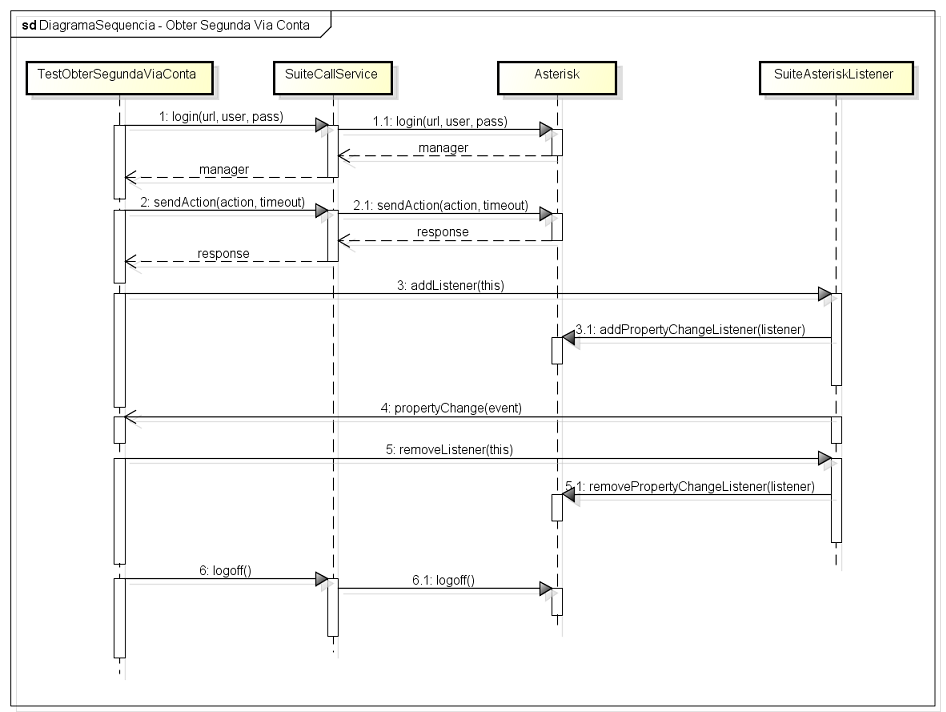
\includegraphics{figuras/diagramaSequenciaObter2ViaTest.png}
	\legend {\fontsize{10}{12}\selectfont {Fonte: Autoria Própria}.}
\end{figure}

Durante a execução de um cenário de teste, é necessário monitorar o comportamento da chamada ou canal internamento na ferramente Asterisk,
afim de validar o retorno obtido pela requisição e posteriormente evidenciar a ocorrência do comportamento esperado ou de falhas. Com isso se faz necessário habilitar a conexão remota na ferramenta Asterisk, no arquivo \textit{/etc/asterisk/manager.conf}.

A distribuição Disc-OS por padrão possui uma configuração de firewall bastante restritiva por questões de segurança, para que não ocorra rejeição nas solicitações realizadas ao Asterisk, será para fins de testes desabilitada as regras do firewall, utilizando o seguinte comando \textit{/etc/init.d/iptables stop}.
 
 Além de desabilitar as regras de firewall será preciso habilitar a c
 
% Figura para demonstrar a classe de teste - classe_teste_suite.png
% Para execução dos testes foi necessário realizar algumas customizações na ferramenta Asterisk, 
% desabilitar o iptables, 
% contexto de teste,
% Criação/Habilitar o user manager para remote conection.
% /etc/asterisk/manager.conf
% [general]
% enabled=yes 
% port=5038
% bindaddr=0.0.0.0
% displayconnects=yes
% permit=0.0.0.0/0.0.0.0

% [manager]
% secret=pa55w0rd 
% allow=0.0.0.0/0.0.0.0
% read=system,call,log,verbose,command,agent,user
% write=system,call,log,verbose,command,agent,user
% permit=0.0.0.0/0.0.0.0



% ----------------------------------------------------------
% PARTE III - RESULTADOS ALCANÇADOS
% ----------------------------------------------------------
%\part{Resultados}
\chapter[Experimentação Utilizando a Suíte de Testes Automatizados]{\textbf{E}xperimentação \textbf{U}tilizando a \textbf{S}uíte de \textbf{T}estes \textbf{A}utomatizados}
%\chapter[Resultados Alcançados]{\textbf{R}esultados \textbf{A}lcançados}
%\addcontentsline{toc}{chapter}{Resultados Alcançados}

\textit{Será apresentado neste capítulo a execução dos experimentos sob a solução abordada nas seções anteriores, e exposto os resultados que foram alcançados.}


\subsection{Preparação do Ambiente de teste}

Os experimentos sobre a solução de integração dos sistemas, foram planejados em um ambiente controlado quanto na elaboração e análise dos cenários de testes envolvidos. 

Para que os cenários de teste sejam o mais semelhante ao ambiente de produção, os mesmos serão executados sobre uma chamada telefônica tendo como originador o suposto cliente com as devidas características. 

O ambiente para execução dos testes será realizando um terminal cujo as especificações estão descritas abaixo:

\begin{table}[htb]
	\footnotesize
	\caption{Recursos computacionais utilizados}
	\label{tabela:recursosUtilizados}
	\begin{tabular}{|p{3.5cm}|p{3cm}|p{2cm}|p{4cm}|} \hline
		\textbf{SISTEMA OPER.} 	& \textbf{PROCESSADOR} 				& \textbf{MEMÓRIA} 	& \textbf{ARMAZENAMENTO}  \\ \hline
		Windows 7 64 bits 		& Intel Core i7-3520M CPU@2.9GHz 	& 8GB DDR3			& 1TB 5400 rpm \\ \hline
	\end{tabular}
	\legend{\fontsize{10}{12}\selectfont {Fonte: Autoria Própria}.}
\end{table}

Este terminal é responsável em executar ambos os sistemas envolvidos, no entanto como o software Asterisk está disponível somente para plataforma Linux, é preciso utilizar o recurso de máquina virtual através do software Virtual Box\footnote{Disponível em \url{https://www.virtualbox.org/}}, para subir uma instância da distribuição Disc-Os conforme citado nas seções anteriores.
 
O terminal possui uma conexão de rede local ativa, para que seja atribuído um endereço IP ao sistema operacional hospedeiro e ao convidado.
Visando garantir o correto funcionamento e a padronização do ambiente de teste foram criados testes de integração reproduzindo uma chamada telefônica programaticamente simulando um ambiente real, para tanto foi necessário utilizar os seguintes recursos o \textit{framework} JUnit na construção dos testes e o recurso nativo do Asterisk chamado \textit{Local Channel} que permite criar um canal de comunicação com um contexto e extensão específica dentro do sistema Asterisk, ou seja permite acessar diretamente o ponto de integração entre os sistemas.

Foram criados contextos\ref{key:contexto} específicos para teste no software Asterisk, replicando os mesmos contextos utilizados no fluxo da URA visando 
isolar o comportamento que ocorre no momento da integração sem a necessidade de redirecionamentos entre serviços ou ramais, conforme visto abaixo;

\begin{figure}[H]
	\centering
	\caption{Declaração dos contextos de teste no Asterisk}
	\label{figura:contextoTeste}
	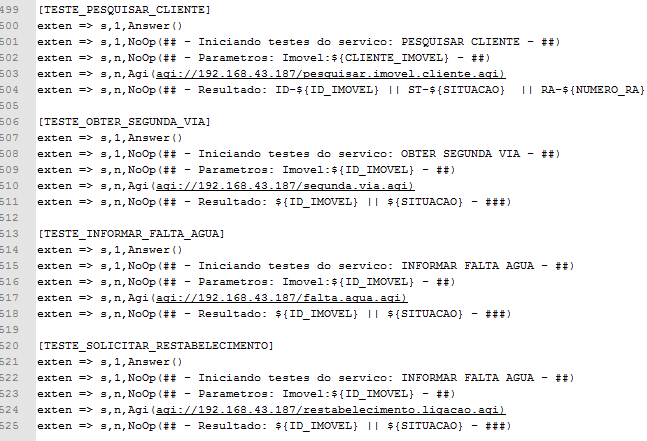
\includegraphics{figuras/contexto_teste.png}
	\legend {\fontsize{10}{12}\selectfont {Fonte: Autoria Própria}.}	
\end{figure}


\subsection{Cenários de Teste}
Nesta fase foram elaborados possíveis cenários de teste para os três serviços automatizados, são respectivamente Obter 2ª via de conta, Informar Falta de Água e Solicitar Restabelecimento da Ligação de Água. Cada serviço proposto possui um objetivo específico sempre vinculado a um imóvel e/ou cliente.
Os cenários de testes representam as possíveis situações cadastrais fictícias e comportamentais vinculadas a um cliente, essencial para realizar um atendimento via sistema. Foram propostos 3 cenários de teste para cada serviço citado acima, visando assegurar o correto comportamento da solução. Abaixo estão descritos os cenários conforme cada serviço proposto:

\subsubsection{Obter 2ª Via de Conta}
Este serviço tem como objetivo checar se há alguma conta pendente referente ao imóvel informado, caso haja pendência o serviço deve submeter a conta pendente via e-mail para o cliente do imóvel. 

Abaixo serão descritos os casos de testes previstos para o serviço obter 2ª Via de Conta, foi cadastrado o mesmo endereço de e-mail para os 3 cenários.
\begin{flushleft}
	\begin{description}
		\item \textbf{CENÁRIO 1}: Cliente devidamente cadastrado no Sistema, atualmente usuário de um imóvel que possui ativo a Ligação de Água e Esgoto, com uma conta em atraso. O Cliente deseja obter a conta em aberto, conforme demostrado na figura \ref{figura:2ViaCenario1}.
		\begin{figure}[H]
			\centering
			\caption{Obter 2ª via - Cenário de Teste 1}
			\label{figura:2ViaCenario1}
			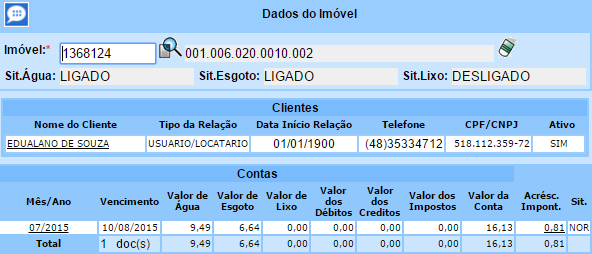
\includegraphics{figuras/cenarios/segunda_via/cenario_1.PNG}
			\legend {\fontsize{10}{12}\selectfont {Fonte: Autoria Própria}.}	
		\end{figure}
	\end{description}
	
	\begin{description}
		\item \textbf{CENÁRIO 2}: Cliente devidamente cadastrado no Sistema, atualmente sendo usuário de um imóvel que possui a Ligação de Água cortada por falta de pagamento, atualmente com três contas em aberto. O Cliente deseja obter a conta de maior atraso, conforme demostrado na figura \ref{figura:2ViaCenario2}.
		\begin{figure}[H]
			\centering
			\caption{Obter 2ª via - Cenário de Teste 2}
			\label{figura:2ViaCenario2}
			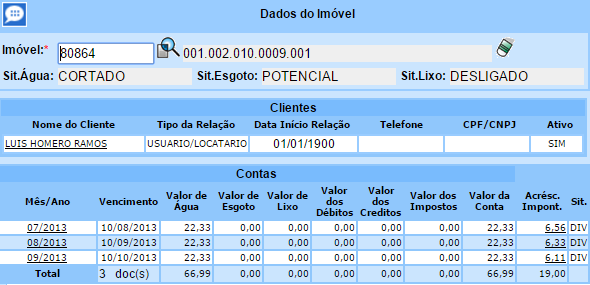
\includegraphics{figuras/cenarios/segunda_via/cenario_2.PNG}
			\legend {\fontsize{10}{12}\selectfont {Fonte: Autoria Própria}.}	
		\end{figure}
	\end{description}
	
	\begin{description}
		\item \textbf{CENÁRIO 3}: Cliente sem e-mail cadastrado no Sistema, atualmente sendo proprietário por dois imóveis que possuem ativo a Ligação de Água, possuindo várias contas pendentes para cada imóvel. O Cliente pretende obter todas as contas de todos os imóveis, conforme demostrado na figura \ref{figura:2ViaCenario3}.
		\begin{figure}[H]
			\centering
			\caption{Obter 2ª via - Cenário de Teste 3}
			\label{figura:2ViaCenario3}
			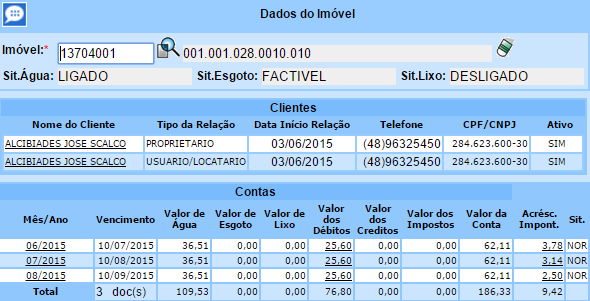
\includegraphics{figuras/cenarios/segunda_via/cenario_3.PNG}
			\legend {\fontsize{10}{12}\selectfont {Fonte: Autoria Própria}.}	
		\end{figure}
	\end{description}
	
\end{flushleft}


\subsubsection{Informar Falta de Água}
Este serviço tem como objetivo formalizar junto ao sistema GSAN um novo Registro de Atendimento referente a Falta de Água para o imóvel informado.
Abaixo serão descritos os casos de testes previstos para o serviço Informar Falta de Água.
\begin{flushleft}
	\begin{description}
		\item \textbf{CENÁRIO 1}: Cliente devidamente cadastrado no Sistema, atualmente locatário de um imóvel que possui ativo a Ligação de Água e Esgoto, com pendência de duas contas, com problemas no abastecimento de água. O Cliente pretende informar a falta de água para o imóvel, conforme demostrado na figura \ref{figura:informarFaltaAguaCenario1}.
		\begin{figure}[H]
			\centering
			\caption{Informar Falta de Água - Cenário de Teste 1}
			\label{figura:informarFaltaAguaCenario1}
			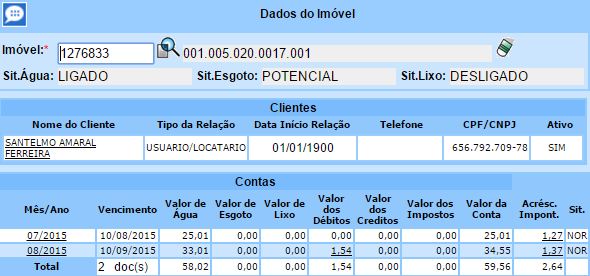
\includegraphics{figuras/cenarios/informar_falta_agua/cenario_1.PNG}
			\legend {\fontsize{10}{12}\selectfont {Fonte: Autoria Própria}.}	
		\end{figure}
	\end{description}
	
	\begin{description}
		\item \textbf{CENÁRIO 2}: Cliente sem e-mail cadastrado no Sistema, atualmente usuário de um único imóvel que possui ativo a Ligação de Água, com situação de adimplência, com problemas no abastecimento de água. O Cliente pretende informar a falta de água para o único imóvel, conforme demostrado na figura \ref{figura:informarFaltaAguaCenario1}.
		\begin{figure}[H]
			\centering
			\caption{Informar Falta de Água - Cenário de Teste 2}
			\label{figura:informarFaltaAguaCenario2}
			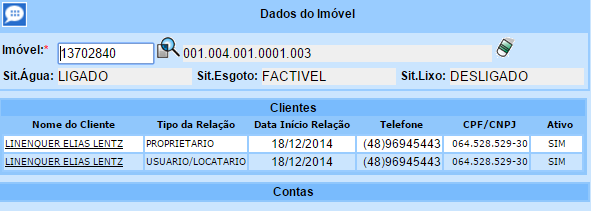
\includegraphics{figuras/cenarios/informar_falta_agua/cenario_2.PNG}
			\legend {\fontsize{10}{12}\selectfont {Fonte: Autoria Própria}.}	
		\end{figure}		
	\end{description}
	
	\begin{description}
		\item \textbf{CENÁRIO 3}: Cliente devidamente cadastrado no Sistema, atualmente proprietário de dois imóveis, que possuem a Ligação de Água ativa, em situação de inadimplência. O Cliente deseja informar problemas no abastecimento de água do imóvel específico onde reside, conforme demostrado na figura \ref{figura:informarFaltaAguaCenario3}.
		\begin{figure}[H]
			\centering
			\caption{Informar Falta de Água - Cenário de Teste 3}
			\label{figura:informarFaltaAguaCenario3}
			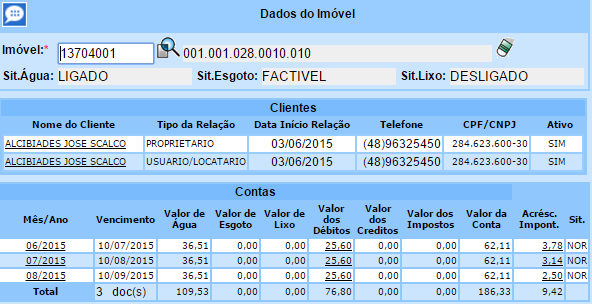
\includegraphics{figuras/cenarios/informar_falta_agua/cenario_3.PNG}
			\legend {\fontsize{10}{12}\selectfont {Fonte: Autoria Própria}.}	
		\end{figure}
	\end{description}
\end{flushleft}	

\subsubsection{Solicitar Restabelecimento da Ligação de Água}
Este serviço tem como objetivo formalizar junto ao sistema GSAN um novo Registro de Atendimento referente ao Restabelecimento da Ligação de Água para um imóvel informado.
Abaixo serão descritos os casos de testes previstos para o serviço Solicitar Restabelecimento da Ligação de Água.
\begin{flushleft}
	\begin{description}
		\item \textbf{CENÁRIO 1}: Cliente devidamente cadastrado no Sistema, atualmente proprietário de um único imóvel que possui a Ligação de Água interrompida por corte, em situação recente de adimplência. O Cliente deseja solicitar restabelecimento da ligação para o imóvel, conforme demostrado na figura \ref{figura:restabelecimentoLigacaoCenario1}.
		\begin{figure}[H]
			\centering
			\caption{Restabelecimento da Ligação de Água - Cenário de Teste 1}
			\label{figura:restabelecimentoLigacaoCenario1}
			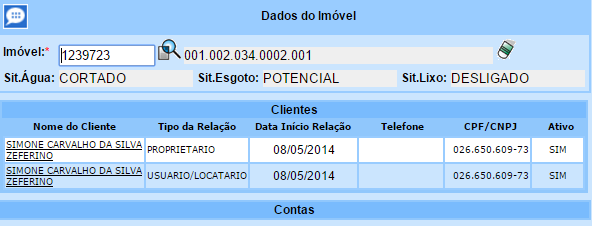
\includegraphics{figuras/cenarios/restabelecimento/cenario_1.PNG}
			\legend {\fontsize{10}{12}\selectfont {Fonte: Autoria Própria}.}	
		\end{figure}
	\end{description}
	
	\begin{description}
		\item \textbf{CENÁRIO 2}: Cliente devidamente cadastrado no Sistema, atualmente usuário de um único imóvel que possui a Ligação de Água interrompida por corte, em situação recente de adimplência. O Cliente deseja solicitar restabelecimento da ligação para o imóvel, conforme demostrado na figura \ref{figura:restabelecimentoLigacaoCenario2}.
		\begin{figure}[H]
			\centering
			\caption{Restabelecimento da Ligação de Água - Cenário de Teste 2}
			\label{figura:restabelecimentoLigacaoCenario2}
			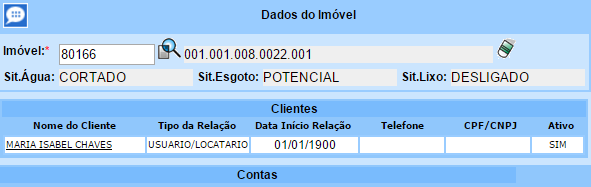
\includegraphics{figuras/cenarios/restabelecimento/cenario_2.PNG}
			\legend {\fontsize{10}{12}\selectfont {Fonte: Autoria Própria}.}	
		\end{figure}
	\end{description}
	
	\begin{description}
		\item \textbf{CENÁRIO 3}: Cliente devidamente cadastrado no Sistema, atualmente proprietário de um imóvel, que possui Ligação de Água interrompida por corte, devido a falta de pagamento das várias contas em aberto. O Cliente deseja solicitar restabelecimento da ligação para o imóvel sem realizar a negociação das faturas, conforme demostrado na figura \ref{figura:restabelecimentoLigacaoCenario3}.
		\begin{figure}[H]
			\centering
			\caption{Restabelecimento da Ligação de Água - Cenário de Teste 3}
			\label{figura:restabelecimentoLigacaoCenario3}
			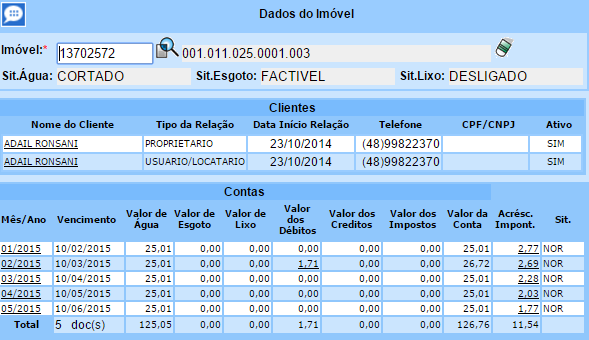
\includegraphics{figuras/cenarios/restabelecimento/cenario_3.PNG}
			\legend {\fontsize{10}{12}\selectfont {Fonte: Autoria Própria}.}	
		\end{figure}
	\end{description}

\end{flushleft}	


\subsection{Execução dos Cenários de Teste}


A execução dos cenários propostos foi realizado utilizando o \textit{framework} de teste JUnit citados na seção anterior, segue abaixo resultado; 

\subsubsection{Obter 2ª Via de Conta}
 
 Após a execução dos cenários de teste implementados para este serviço foi possível notar que 2/3 Cenários concluíram com sucesso e apenas 1/3 falhou em sua execução, conforme demostrado na figura \ref{figura:segundaViaJUnit}.		
	\begin{figure}[H]
		\centering
		\caption{Obter 2ª Via de Conta - Detalhes execução dos testes}
		\label{figura:segundaViaJUnit}
		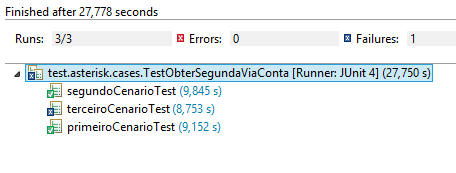
\includegraphics{figuras/cenarios/segunda_via/junit_result.PNG}
		\legend {\fontsize{10}{12}\selectfont {Fonte: Autoria Própria}.}	
	\end{figure}
	

Em cada cenário de teste o sistema deve enviar um e-mail contendo a 2ª via da conta solicitada, a figura \ref{figura:emailRecebido} ilustra a caixa de entrada do E-mail configurado para cada cliente.
	\begin{figure}[H]
		\centering
		\caption{Obter 2ª Via de Conta - E-mail recebido pelo cliente}
		\label{figura:emailRecebido}
		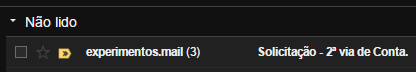
\includegraphics{figuras/cenarios/segunda_via/envio_email.PNG}
		\legend {\fontsize{10}{12}\selectfont {Fonte: Autoria Própria}.}	
	\end{figure}

	
\subsubsection{Informar Falta de Água}

 Após a execução dos cenários de teste implementados para este serviço foi possível identificar que todos os 3 cenários previsto executaram com sucesso, conforme demostrado na figura \ref{figura:informarFaltaJUnit}.	

	\begin{figure}[H]
		\centering
		\caption{Informar Falta de Água - Detalhes execução dos testes}
		\label{figura:informarFaltaJUnit}
		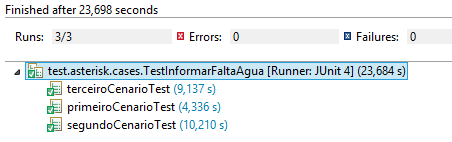
\includegraphics{figuras/cenarios/informar_falta_agua/junit_result.PNG}
		\legend {\fontsize{10}{12}\selectfont {Fonte: Autoria Própria}.}	
	\end{figure}

Ao consulta o sistema GSAN, visando identificar se houve a ocorrência da formalização dos Registros de Atendimentos, o primeiro cenário cujo o identificar 1276833 representa a matrícula do imóvel, houve a geração do Registro de Atendimento de número 6594, conforme demonstrado na figura \ref{figura:informarFaltaRA1}.

	\begin{figure}[H]
		\centering
		\caption{Informar Falta de Água - RA gerado para o Cenário 1}
		\label{figura:informarFaltaRA1}
		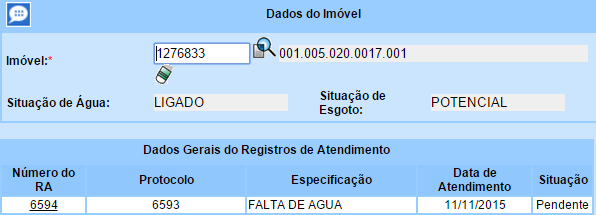
\includegraphics{figuras/cenarios/informar_falta_agua/resultado_1.PNG}
		\legend {\fontsize{10}{12}\selectfont {Fonte: Autoria Própria}.}	
	\end{figure}
	
Para o segundo cenário, cujo o identificador 13702840 representa a matrícula do imóvel, houve a geração do Registro de Atendimento de número 6598, conforme exposto na figura \ref{figura:informarFaltaRA2}.	
		
	\begin{figure}[H]
		\centering
		\caption{Informar Falta de Água - RA gerado para o Cenário 2}
		\label{figura:informarFaltaRA2}
		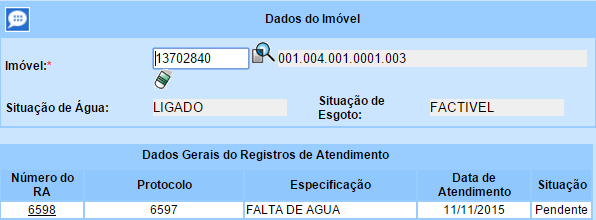
\includegraphics{figuras/cenarios/informar_falta_agua/resultado_2.PNG}
		\legend {\fontsize{10}{12}\selectfont {Fonte: Autoria Própria}.}	
	\end{figure}

Para o terceiro cenário, cujo o identificador 13704001 representa a matrícula do imóvel, também houve a geração do Registro de Atendimento de número 6596, conforme exposto na figura \ref{figura:informarFaltaRA3}.	

\begin{figure}[H]
	\centering
	\caption{Informar Falta de Água - RA gerado para o Cenário 3}
	\label{figura:informarFaltaRA3}
	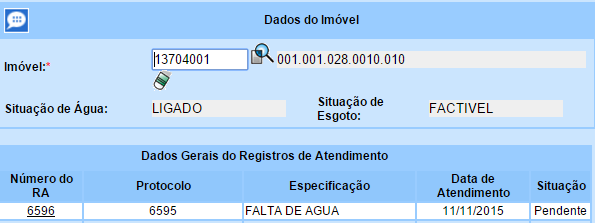
\includegraphics{figuras/cenarios/informar_falta_agua/resultado_3.PNG}
	\legend {\fontsize{10}{12}\selectfont {Fonte: Autoria Própria}.}	
\end{figure}	

		
\subsubsection{Solicitar Restabelecimento da Ligação de Água}

 Após a execução dos cenários de teste implementados para este serviço foi possível identificar que todos os 3 cenários previsto executaram com sucesso, conforme demostrado na figura \ref{figura:restabelecimentoJUnit}.	

\begin{figure}[H]
	\centering
	\caption{Restabelecimento da Ligação de Água - Detalhes execução dos testes}
	\label{figura:restabelecimentoJUnit}
	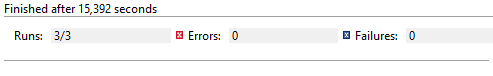
\includegraphics{figuras/cenarios/restabelecimento/junit_result.PNG}
	\legend {\fontsize{10}{12}\selectfont {Fonte: Autoria Própria}.}	
\end{figure}

Ao consulta o sistema GSAN, visando identificar se houve a ocorrência da formalização dos Registros de Atendimentos, o primeiro cenário cujo o identificar 1239723 representa a matrícula do imóvel, houve a geração do Registro de Atendimento de número 6604, conforme demonstrado na figura \ref{figura:restabelecimentoRA1}.

\begin{figure}[H]
	\centering
	\caption{Restabelecimento da Ligação de Água - RA gerado para o Cenário 1}
	\label{figura:restabelecimentoRA1}
	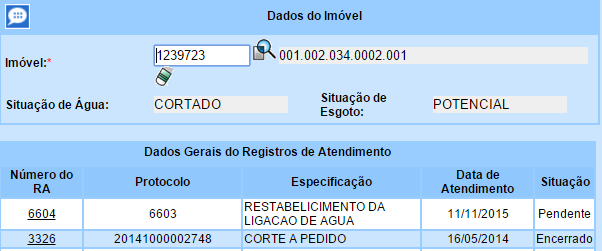
\includegraphics{figuras/cenarios/restabelecimento/resultado_1.PNG}
	\legend {\fontsize{10}{12}\selectfont {Fonte: Autoria Própria}.}	
\end{figure}

Para o segundo cenário, cujo o identificador 80166 representa a matrícula do imóvel, houve a geração do Registro de Atendimento de número 6608, conforme exposto na figura \ref{figura:restabelecimentoRA2}.	

\begin{figure}[H]
	\centering
	\caption{Restabelecimento da Ligação de Água - RA gerado para o Cenário 2}
	\label{figura:restabelecimentoRA2}
	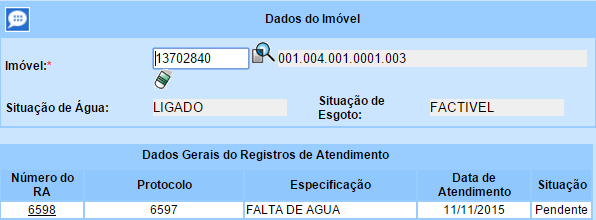
\includegraphics{figuras/cenarios/informar_falta_agua/resultado_2.PNG}
	\legend {\fontsize{10}{12}\selectfont {Fonte: Autoria Própria}.}	
\end{figure}
	
Para o terceiro cenário, cujo o identificador 13702572 representa a matrícula do imóvel, mesmo o cliente em situação de inadimplência houve a geração do Registro de Atendimento de número 6606, conforme exposto na figura \ref{figura:restabelecimentoRA3}.	

\begin{figure}[H]
	\centering
	\caption{Restabelecimento da Ligação de Água - RA gerado para o Cenário 3}
	\label{figura:restabelecimentoRA3}
	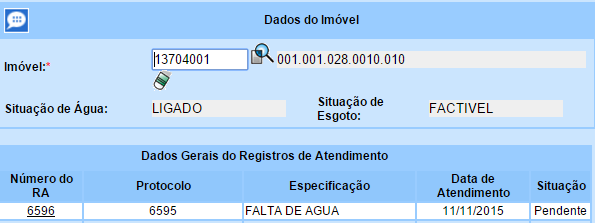
\includegraphics{figuras/cenarios/informar_falta_agua/resultado_3.PNG}
	\legend {\fontsize{10}{12}\selectfont {Fonte: Autoria Própria}.}	
\end{figure}	

Os detalhes sobre cada Registro de Atendimento mencionado acima podem ser consultados nos anexos deste trabalho.



% Conclusao
%\section{Resultado dos Cenários de Teste}

Após a apuração dos cenários descritos acima, chegamos aos seguintes resultados por serviço:

\begin{table}[H]
	\center
	\footnotesize
	\caption{Avaliação do serviço 2ª via de Conta }
	\label{tabela:avaliacaoSegundaViaConta}
	\begin{tabular}{|p{3cm}|p{3cm}|p{3cm}|}
		\hline
		\multicolumn{3}{|c|}{\textbf{2ª via de Conta}} \\
		\hline
		\textbf{Cenários}  	& \textbf{Situação} & \textbf{Percentual (\%)}  \\
		\hline		
		Cenário 1			& SUCESSO 		& (+) 33,33\% 	\\
		\hline
		Cenário 2 			& SUCESSO		& (+) 33,33\% 	\\
		\hline
		Cenário 3 			& FALHA 		& (+) 33,33\%	\\
		\hline		
		\multicolumn{2}{|c|}{\textbf{TOTAL}}	& 66\% 	\\
		\hline				
	\end{tabular}
	\legend{\fontsize{10}{12}\selectfont {Fonte: Autoria Própria}.}
\end{table}

O serviço de obter 2ª via de conta obteve o percentual de 66\% de sucesso nos cenários de testes aplicados sobre o produto gerado, conforme demostra a tabela \ref{tabela:avaliacaoSegundaViaConta}. 


\begin{table}[H]
	\center
	\footnotesize
	\caption{Informar Falta de Água}
	\label{tabela:avaliacaoInformarFaltaAgua}
	\begin{tabular}{|p{3cm}|p{3cm}|p{3cm}|}
		\hline
		\multicolumn{3}{|c|}{\textbf{Informar Falta de Água}} \\
		\hline
		\textbf{Cenários}  	& \textbf{Situação} & \textbf{Percentual (\%)}  \\
		\hline		
		Cenário 1			& SUCESSO 		& (+) 33,33\% 	\\
		\hline
		Cenário 2 			& SUCESSO		& (+) 33,33\% 	\\
		\hline
		Cenário 3 			& SUCESSO 		& (+) 33,33\%	\\
		\hline		
		\multicolumn{2}{|c|}{\textbf{TOTAL}}	& 100\% 	\\
		\hline				
	\end{tabular}
	\legend{\fontsize{10}{12}\selectfont {Fonte: Autoria Própria}.}
\end{table}

O serviço de Informar Falta de Água obteve o percentual de 100\% de sucesso nos cenários de testes aplicados sobre o produto gerado, conforme demostra a tabela \ref{tabela:avaliacaoInformarFaltaAgua}.


\begin{table}[H]
	\center
	\footnotesize
	\caption{Solicitar Restabelecimento da Ligação}
	\label{tabela:avaliacaoRestabelerLigacaoAgua}
	\begin{tabular}{|p{3cm}|p{3cm}|p{3cm}|}
		\hline
		\multicolumn{3}{|c|}{\textbf{Solicitar Restabelecimento da Ligação}} \\
		\hline
		\textbf{Cenários}  	& \textbf{Situação} & \textbf{Percentual (\%)}  \\
		\hline		
		Cenário 1			& SUCESSO 		& (+) 33,33\% 	\\
		\hline
		Cenário 2 			& SUCESSO		& (+) 33,33\% 	\\
		\hline
		Cenário 3 			& SUCESSO 		& (+) 33,33\%	\\
		\hline		
		\multicolumn{2}{|c|}{\textbf{TOTAL}}	& 100\% 	\\
		\hline				
	\end{tabular}
	\legend{\fontsize{10}{12}\selectfont {Fonte: Autoria Própria}.}
\end{table}

O serviço de Solicitar Restabelecimento da Ligação obteve o percentual de 100\% de sucesso nos cenários de testes aplicados sobre o produto gerado, conforme demostra a tabela \ref{tabela:avaliacaoRestabelerLigacaoAgua}.



\section{Apresentação dos Resultados Obtidos}

Levando em consideração os resultados obtidos através da aplicação de todos os cenários de testes descritos acima sob os serviços desenvolvidos neste trabalho,
é possível afirmar que a utilização da uma URA para realizar o atendimento de primeiro nível tem potencial para reduzir parte dos atendimentos destinados à solicitação de 2ª via de conta, falta de água e restabelecimento da ligação, definindo na padronização dos atendimentos e contribuindo para a redução dos custos.
 
 %observando os percentuais atingidos com base na média descrita dos principais %Serviços do Atendimento ao Público, notamos que a solução proposta é capaz de %reduzir em até 20,46\%, dos registros de atendimentos diários, conforme visto %abaixo na figura \ref{figura:eficienciaServicos}:	

%\begin{figure}[!htb]
%	\centering
%	\caption{Gráfico de avaliação dos serviços automatizados}
%	\label{figura:eficienciaServicos}	
%	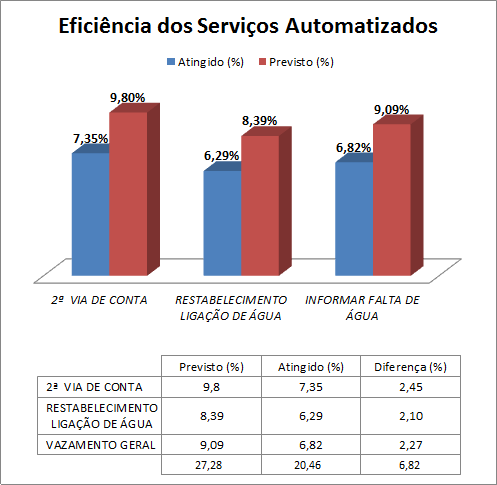
\includegraphics{figuras/eficiencia_servicos.png}
%	\legend {\fontsize{10}{12}\selectfont {Fonte: Autoria Própria}.}
%\end{figure}


\chapter[Considerações Finais e Trabalhos Futuros]{\textbf{C}onsiderações Finais e \textbf{T}rabalhos Futuros}
\addcontentsline{toc}{chapter}{Considerações Finais e Trabalhos Futuros}

A solução em \textit{software} apresentada e desenvolvida se trata de uma proposta inicial que pode se tornar um módulo interno com grandes potenciais para integrações futuras, neste trabalho foi adotada a integração do sistema GSAN com uma central de atendimento automatizada através do \textit{software} Asterisk, os novos serviços desenvolvidos possibilitam a reutilização para quaisquer outras soluções do gênero, o código fonte será disponibilizado na comunidade do GSAN, para que seja mantido e evoluído ao longo do tempo. Existem alguns recursos ou rotinas que podem ser criados para melhor aproveitamento e aprimoramento da solução proposta.

\begin{itemize}
	\item Reconhecimento de voz, para os casos de falta de água, que ocorre em regiões fora do endereço do cliente, de forma que o cliente possa informar a Rua que ocorre o problema.
	\item Automatizar serviços como negociação de débitos do cliente para serem realizados através da URA.
	\item Automatizar o \textit{feedback} dos serviços realizados, ou seja, a cada térmico de Ordem de Serviço o GSAN solicita do Asterisk que ele contate o cliente.
	\item Utilizar o Interceptador gerando estatísticas dos acessos realizados, coletando tempo de respostas e traçando perfis de cliente que mais realizam solicitações via \textit{Call Center}.
\end{itemize}

Estes são cenários que podem contribuir para o melhor aproveitamento da solução, com potencial de redução ainda maior dos registros de atendimentos. 



% ----------------------------------------------------------
% Finaliza a parte no bookmark do PDF para que se inicie o bookmark na raiz e adiciona espaço de parte no Sumário
% ----------------------------------------------------------
\phantompart
% ----------------------------------------------------------
% ELEMENTOS PÓS-TEXTUAIS
% ----------------------------------------------------------
\postextual

% Referências bibliográficas
\bibliography{bibtex/referencias}

% Glossário (Consulte o manual da classe abntex2 para orientações sobre o glossário)
%\glossary

% Apêndices
%\begin{apendicesenv}
	
	\partapendices

\chapter{Processo de configuração da JDK na IDE de desenvolvimento}

O sistema GSAN roda sob a JDK (\textit{Java Develop Kit}) 5, disponível atualmente no site da Oracle Coportarion, sendo necessário configurar a IDE com a versão correta para compilar o projeto, podemos configurar facilmente acessando a opção no menu superior \textit{Window > Preferences > Java > Installed JREs} em seguida será preciso adicionar uma nova JVM (\textit{Java Virtual Machine}) selecionando a opção Add e selecionar a opção Standard VM, conforme visto na figura \ref{figura:anexo1};

\begin{figure}[H]
	\centering
	\caption*{\textbf{Selecionar Tipo de JVM.}}
	\label{figura:anexo1}
	\begin{subfigure}[H]{\textwidth}
		\centering
		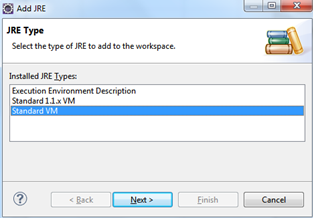
\includegraphics{figuras/anexo/selectJVM.png}
		\legend {\fontsize{10}{12}\selectfont {Fonte: Autoria Própria}.}	
	\end{subfigure}
\end{figure}


Após a seleção é preciso confirmar a ação clicando em Next, na nova janela exibida o botão Directory... permite localizar o diretório onde está a versão do JDK que será utilizada, dessa forma deve ser selecionado o diretório raiz da versão, no exemplo representado por \textit{C:/pessoal/java/jdk1.5.0\_22}, conforme visto na figura \ref{figura:anexo2};

\begin{figure}[H]
	\centering
	\caption*{\textbf{Adicionar nova JRE na IDE.}}
	\label{figura:anexo2}
	\begin{subfigure}[H]{\textwidth}
		\centering
		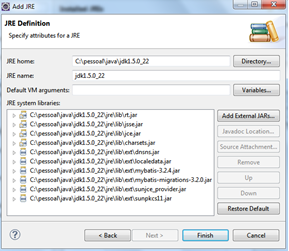
\includegraphics{figuras/anexo/addJRE.png}
		\legend {\fontsize{10}{12}\selectfont {Fonte: Autoria Própria}.}	
	\end{subfigure}
\end{figure}

A própria IDE já preenche o JRE name, caso isso não ocorra será necessário preencher este campo de preferência com o nome da versão do JDK utilizada, realizado este passo a IDE terá condições de compilar as instruções contidas no fonte.  Com isso será necessário importa o projeto no GSAN na IDE de desenvolvimento, selecionando a opção \textit{File > Import..}, abrirá um janela onde deve ser selecionando a opção \textit{General > Existing Projects into Workspace}, em seguida através do botão \textit{Browser} será possível localizar o diretório onde está o fonte do sistema GSAN, conforme ilustrado na figura \ref{figura:anexo3};

\begin{figure}[H]
	\centering
	\caption*{\textbf{Importar Sistema GSAN na IDE.}}
	\label{figura:anexo3}
	\begin{subfigure}[H]{\textwidth}
		\centering
		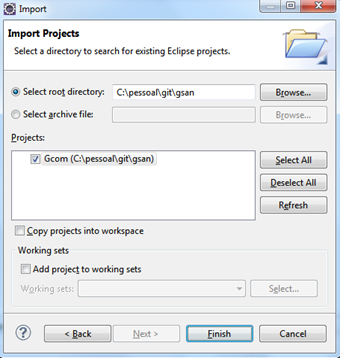
\includegraphics{figuras/anexo/importGSAN.png}
		\legend {\fontsize{10}{12}\selectfont {Fonte: Autoria Própria}.}	
	\end{subfigure}
\end{figure}


Feito isso precisa somente pressionar o botão de \textit{Finish}, para confirmar a importação do projeto para a IDE de desenvolvimento.

\chapter{Configurar variável de ambiente do servidor de aplicação Jboss}

Neste trabalho foi utilizado o projeto \textit{Open Source Jboss Community} na versão 4.0.1, compatível com as tecnologias utilizadas no GSAN, para utilizá-lo será preciso declarar uma variável de ambiente no sistema operacional, por padrão nomeado de JBOSS\_HOME contendo a localização do diretório do servidor de aplicação, no exemplo abaixo representado por \textit{C:/pessoal/jboss/jboss-4.0.1sp1}, conforme visto na figura \ref{figura:anexo4};

\begin{figure}[H]
	\centering
	\caption*{\textbf{Adicionando variável de ambiente JBOSS\_HOME.}}
	\label{figura:anexo4}
	\begin{subfigure}[H]{\textwidth}
		\centering
		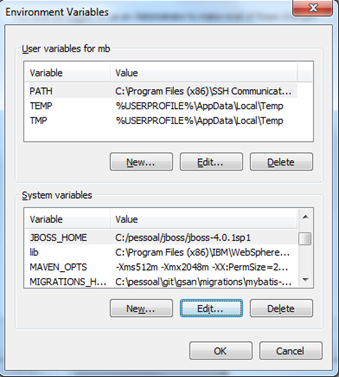
\includegraphics{figuras/anexo/var_JBOSS_HOME.png}
		\legend {\fontsize{10}{12}\selectfont {Fonte: Autoria Própria}.}	
	\end{subfigure}
\end{figure}


Após a criação desta variável de ambiente, será preciso atualizar a variável de ambiente chamada PATH que reúne as variáveis utilizadas no sistema operacional, adicionando ao final o seguinte texto \textit{\%JBOSS\_HOME\%/bin;} para que o sistema operacional consiga localizar o diretório /bin do servidor de aplicação que contém o script de inicialização do servidor chamado \textit{run.bat} para sistemas Windows e \textit{run.sh} para sistemas Unix, neste script é possível modificar os parâmetros utilizados na execução do servidor de aplicação sob a JVM para a alocação de memória assim como habilitar a utilização de técnicas de debug remoto das aplicações.


\chapter{Configuração do Fluxo da URA}
Segue abaixo a configuração do fluxo completo da URA, configurado no seguinte arquivo de configuração \textit{/etc/asterisk/extension.conf};
\\\\
; Declarando o contexto de boas vindas para executar o áudio ‘inicial’ \\
; o dígito representa a rotina associada abaixo: \\
; 1 – Contexto de identificação do Cliente. \\
; 2 – Falar com o atendente. \\
\textbf{[disc-ivr-BOAS\_VINDAS] }	 \\
exten => s,1,Playback(custom/inicial)  \\
exten => 1,1,Goto(disc-ivr-IDENTIFICACAO,7001,1)  \\
exten => 2,1,Goto(FALAR\_ATENDENTE,s,1)  \\
 \\
; Declarando o contexto de identificação do cliente, executa o áudio  \\
; ‘identificacao’ e redireciona para o contexto de PESQUISAR\_CLIENTE \\
; executa o áudio ‘pronto’ e ‘numero\_ra’, soletra o numero do RA e  \\
; direciona para o Menu principal. \\
\textbf{[disc-ivr-IDENTIFICACAO]} \\
exten => 7001,1,Playback(custom/identificacao) \\
exten => 7001,2,Goto(PESQUISAR\_CLIENTE,s,1) \\
exten => 7001,3,Playback(custom/pronto) \\
exten => 7001,4,Playback(custom/numero\_ra) \\
exten => 7001,5,SayDigits(\${NUMERO\_RA}) \\
exten => 7001,6,Goto(disc-ivr-MENU,7002,1) \\
 \\
; Declara o context do Menu Principal, executa o áudio ‘menu’, \\
; o dígito representa a rotina associada abaixo: \\
; 1 – Serviço de 2ª via de Conta \\
; 2 – Serviço de Informar Falta de Água \\
; 3 – Serviço de Solicitar Restabelecimento da Ligação \\
; 4 – Falar com o atendente. \\
\textbf{[disc-ivr-MENU]} \\
exten => 7002,1,Playback(custom/menu) \\
exten => 1,1,Goto(disc-ivr-2VIA,7003,1) \\
exten => 2,1,Goto(disc-ivr-INFORMAR\_FALTA\_AGUA,7004,1) \\
exten => 3,1,Goto(disc-ivr-SOLICITAR\_RESTABELECIMENTO,7005,1) \\
exten => 4,1,Goto(FALAR\_ATENDENTE,s,1) \\
 \\
; Declarando o contexto de 2ª via, executa o aúdio ‘2via’ \\
; redireciona para o contexto de obter segunda via e \\
; desliga a ligação. \\
\textbf{[disc-ivr-2VIA]} \\
exten => 7003,1,Playback(custom/2via) \\
exten => 7003,2,Goto(OBTER\_SEGUNDA\_VIA,s,1) \\
exten => 7003,3,Hangup() \\
 \\
; Declarando o contexto disc-ivr-INFORMAR\_FALTA\_AGUA \\
; Executa o áudio ‘falta\_agua\_abrir\_chamado’  \\
; Redireciona para o contexto INFORMAR\_FALTA\_AGUA \\
; Executa o áudio ‘sucesso’ \\
; Desliga a ligação \\
\textbf{[disc-ivr-INFORMAR\_FALTA\_AGUA]} \\
exten => 7004,1,Playback(custom/falta\_agua\_abrir\_chamado) \\
exten => 7004,2,Goto(INFORMAR\_FALTA\_AGUA,s,1) \\
exten => 7004,3,Playback(custom/sucesso) \\
exten => 7004,4,Hangup() \\
 \\
; Declarando o contexto disc-ivr-SOLICITAR\_RESTABELECIMENTO \\
; Executa o áudio ‘restabelecimento’  \\
; Redireciona para o contexto SOLICITAR\_RESTABELECIMENTO \\
; Executa o áudio ‘sucesso’ \\
; Desliga a ligação \\
\textbf{[disc-ivr-SOLICITAR\_RESTABELECIMENTO]} \\
exten => 7005,1,Playback(custom/restabelecimento) \\
exten => 7005,2,Goto(SOLICITAR\_RESTABELECIMENTO,s,1) \\
exten => 7005,3,Playback(custom/sucesso) \\
exten => 7005,4,Hangup() \\
 \\
; Declarando o contexto ‘PESQUISAR\_CLIENTE’ \\
; Atende a ligação \\
; Executa o áudio ‘beep’ \\
; Defini o tempo limite de espera entre a discagem dos dígitos \\
; Defini o tempo limite de espera do primeiro dígito \\
; Ler os digitos informados \\
; Cria a variável ‘CLIENTE\_IMOVEL’ recebendo os digitos. \\
; Executa uma requisição Agi para ‘192.168.43.2/pesquisar.imovel.cliente.agi’ \\
; Exibe o ID\_IMOVEL \\
; Verifica a situação da requisição realizada \\
; Caso seja ‘SUCESSO’ redireciona para o contexto disc-ivr-IDENTIFICACAO \\
; Caso seja diferente de sucesso redireciona para FALAR\_ATENDENTE \\
\textbf{[PESQUISAR\_CLIENTE]} \\
exten => s,1,Answer() \\
exten => s,n,PlayBack(beep) \\
exten => s,n,Set(TIMEOUT(digit)=3)  \\
exten => s,n,Set(TIMEOUT(response)=7)  \\
exten => s,n,Read(NUMERO) ; LER OS DIGITOS \\
exten => s,n,Set(CLIENTE\_IMOVEL=\${NUMERO}) \\
exten => s,n,Agi(agi://192.168.43.2/pesquisar.imovel.cliente.agi) \\
exten => s,n,NoOp(\${ID\_IMOVEL}) \\
exten => s,n,GotoIf(\$["\${SITUACAO}" == "SUCESSO"]?ok:falha) \\
exten => s,n(ok),Goto(disc-ivr-IDENTIFICACAO,7001,3) \\
exten => s,n(falha),Goto(FALAR\_ATENDENTE,s,1) \\
 \\
; Declarando o contexto ‘OBTER\_SEGUNDA\_VIA’ \\
; Atende a ligação \\
; Executa uma requisição Agi para ‘192.168.43.2/segunda.via.agi’ \\
; Printa o ‘ID\_IMOVEL’ \\
; Verifica a situação da requisição realizada \\
; Caso seja ‘SUCESSO’ redireciona para o contexto ‘disc-ivr-2VIA’ \\
; Caso seja diferente de sucesso redireciona para ‘FALAR\_ATENDENTE’ \\
\textbf{[OBTER\_SEGUNDA\_VIA]} \\
exten => s,1,Answer() \\
exten => s,n,Agi(agi://192.168.43.2/segunda.via.agi) \\
exten => s,n,NoOp(\${ID\_IMOVEL}) \\
exten => s,n,GotoIf(\$["\${SITUACAO}" == "SUCESSO"]?ok:falha) \\
exten => s,n(ok),Goto(disc-ivr-2VIA,7003,3) \\
exten => s,n(falha),Goto(FALAR\_ATENDENTE,s,1) \\
\\
; Declarando o contexto ‘INFORMAR\_FALTA\_AGUA’ \\
; Atende a ligação \\
; Executa uma requisição Agi para ‘192.168.43.2/falta.agua.agi’ \\
; Verifica a situação da requisição realizada \\
; Caso seja ‘SUCESSO’ redireciona para o contexto \\
; ‘disc-ivr-NFORMAR\_FALTA\_AGUA’ \\
; Caso seja diferente de sucesso redireciona para ‘FALAR\_ATENDENTE’ \\
\textbf{[INFORMAR\_FALTA\_AGUA]} \\
exten => s,1,Answer() \\
exten => s,n,Agi(agi://192.168.43.2/falta.agua.agi) \\
exten => s,n,GotoIf(\$["\${SITUACAO}" == "SUCESSO"]?ok:falha) \\
exten => s,n(ok),Goto(disc-ivr-INFORMAR\_FALTA\_AGUA,7004,3) \\
exten => s,n(falha),Goto(FALAR\_ATENDENTE,s,1) \\
 \\
; Declarando o contexto ‘SOLICITAR\_RESTABELECIMENTO’ \\
; Atende a ligação \\
; Executa uma requisição Agi para ‘192.168.43.2/restabelecimento.ligacao.agi’ \\
; Verifica a situação da requisição realizada \\
; Caso seja ‘SUCESSO’ redireciona p/ o contexto \\
; ‘disc-ivr-SOLICITAR\_RESTABELECIMENTO \\
; Caso seja diferente de sucesso redireciona para ‘FALAR\_ATENDENTE’ \\
\textbf{[SOLICITAR\_RESTABELECIMENTO]} \\
exten => s,1,Answer() \\
exten => s,n,Agi(agi://192.168.43.2/restabelecimento.ligacao.agi) \\
exten => s,n,GotoIf(\$["\${SITUACAO}" == "SUCESSO"]?ok:falha) \\
exten => s,n(ok),Goto(disc-ivr-SOLICITAR\_RESTABELECIMENTO,7005,3) \\
exten => s,n(falha),Goto(FALAR\_ATENDENTE,s,1) \\
 \\
; Declarando o contexto ‘FALAR\_ATENDENTE’ \\
; Executa o áudio ‘ligacao\_redirecionada’ \\
; Realiza uma ligação para o ‘ATENDENTE’ \\
\textbf{[FALAR\_ATENDENTE]} \\
exten => s,1,PlayBack(custom/ligacao\_redirecionada) \\
exten => s,2,Dial(SIP/ATENDENTE) \\


\chapter{Registros de Atendimentos Gerados}

A execução dos cenários de testes resultaram na criação dos seguintes Registros de Atendimentos no sistema GSAN,
a seguir pode ser consultado o detalhamento sobre os Registros de Atendimentos gerados para o serviço Informar Falta de Água.
\begin{figure}[H]
	\centering
	\caption*{\textbf{Informar Falta de Água - Cenário 1 Detalhado.}}
	\begin{subfigure}[H]{\textwidth}
		\centering
		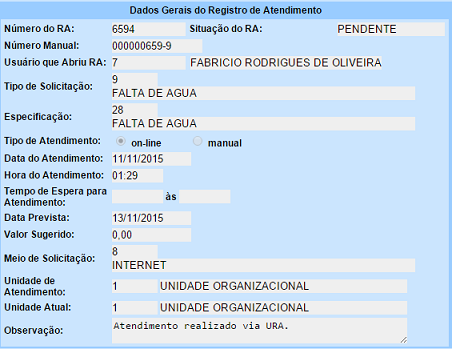
\includegraphics{figuras/anexo/falta_agua/detalhe_1.png}
		\legend {\fontsize{10}{12}\selectfont {Fonte: Autoria Própria}.}	
	\end{subfigure}
\end{figure}

\begin{figure}[H]
	\centering
	\caption*{\textbf{Informar Falta de Água - Cenário 2 Detalhado.}}
	\begin{subfigure}[H]{\textwidth}
		\centering
		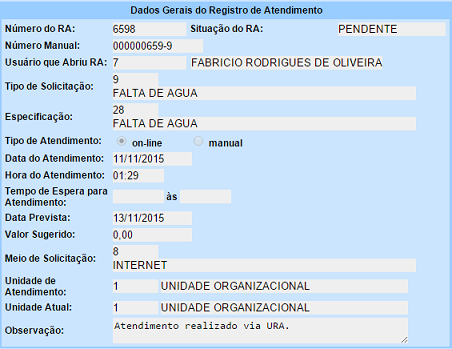
\includegraphics{figuras/anexo/falta_agua/detalhe_2.png}
		\legend {\fontsize{10}{12}\selectfont {Fonte: Autoria Própria}.}	
	\end{subfigure}
\end{figure}

\begin{figure}[H]
	\centering
	\caption*{\textbf{Informar Falta de Água - Cenário 3 Detalhado.}}
	\begin{subfigure}[H]{\textwidth}
		\centering
		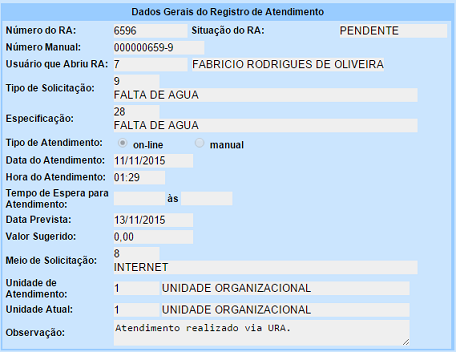
\includegraphics{figuras/anexo/falta_agua/detalhe_3.png}
		\legend {\fontsize{10}{12}\selectfont {Fonte: Autoria Própria}.}	
	\end{subfigure}
\end{figure}



A seguir pode ser consultado os registros de atendimentos abertos pela execução da suíte de testes automatizados para o serviço Solicitar Restabelecimento da Ligação de Água;

\begin{figure}[H]
	\centering
	\caption*{\textbf{Solicitar Restabelecimento da Ligação de Água - Cenário 1 Detalhado.}}
	\begin{subfigure}[H]{\textwidth}
		\centering
		\includegraphics{figuras/anexo/restabelecer/detalhe_1.png}
		\legend {\fontsize{10}{12}\selectfont {Fonte: Autoria Própria}.}	
	\end{subfigure}
\end{figure}

\begin{figure}[H]
	\centering
	\caption*{\textbf{Solicitar Restabelecimento da Ligação de Água - Cenário 2 Detalhado.}}
	\begin{subfigure}[H]{\textwidth}
		\centering
		\includegraphics{figuras/anexo/restabelecer/detalhe_2.png}
		\legend {\fontsize{10}{12}\selectfont {Fonte: Autoria Própria}.}	
	\end{subfigure}
\end{figure}

\begin{figure}[H]
	\centering
	\caption*{\textbf{Solicitar Restabelecimento da Ligação de Água - Cenário 3 Detalhado.}}
	\begin{subfigure}[H]{\textwidth}
		\centering
		\includegraphics{figuras/anexo/restabelecer/detalhe_3.png}
		\legend {\fontsize{10}{12}\selectfont {Fonte: Autoria Própria}.}	
	\end{subfigure}
\end{figure}


\end{apendicesenv}





% Anexos
\begin{anexosenv}

\partanexos

\chapter{Primeiro Anexo}

Texto do primeiro anexo.

\chapter{Segundo Anexo}

Texto do segundo anexo.

\end{anexosenv}



%---------------------------------------------------------------------
% INDICE REMISSIVO
%---------------------------------------------------------------------
\phantompart
\printindex
%---------------------------------------------------------------------
\end{document}
